
%\documentclass[12pt,notitlepage,aps,pra,longbibliography,nofootinbib,tightenlines]{revtex4}
%\documentclass[12pt,notitlepage,longbibliography,nofootinbib,tightenlines]{revtex4-1}

\documentclass[12pt]{article}

%\documentclass[12pt,a4]{revtex4}
%\documentclass[12pt]{article}
%\documentclass[11pt, twocolumn]{article}

%\usepackage{epsf}
\usepackage{amsmath}
\usepackage{color}
\usepackage{natbib}
%\usepackage{cite}
\usepackage{fullpage} % uses 20 percent less pages.

\usepackage{framed}

\RequirePackage{amsmath}
\RequirePackage{amssymb}
\RequirePackage{amsthm}
%\RequirePackage{algorithmic}
%\RequirePackage{algorithm}
%\RequirePackage{theorem}
%\RequirePackage{eucal}
\RequirePackage{color}
\RequirePackage{xcolor}
\RequirePackage{url}
\RequirePackage{mdwlist}

\RequirePackage[all]{xy}
\CompileMatrices
\RequirePackage{hyperref}
\RequirePackage{graphicx}
%\RequirePackage[dvips]{geometry}

\newtheorem{theorem}{Theorem}
\newtheorem{lemma}{Lemma}

%\renewenvironment{framed}[1][\hsize]{%
%\def\FrameCommand{{\color{red}\vrule width 3pt}\hspace{0pt}\fboxsep=\FrameSep\colorbox{yellow}}%
%\MakeFramed{\hsize#1\advance\hsize-\width\FrameRestore}}
%{\endMakeFramed}

%\renewenvironment{framed}[1][\hsize]{%
%\def\FrameCommand{{\color{red}\vrule width 3pt}\hspace{0pt}\fboxsep=\FrameSep\colorbox{yellow}}%
%\MakeFramed{\hsize0.8\linewidth\advance\hsize-\width\FrameRestore}}
%{\endMakeFramed}

\renewenvironment{framed}[1][\hsize]{%
\def\FrameCommand{{\color{black}\vrule width 3pt}\hspace{0pt}\fboxsep=\FrameSep\colorbox{lightgray}}%
\MakeFramed{\hsize0.8\linewidth\advance\hsize-\width\FrameRestore}}
{\endMakeFramed}


\begin{document}

%\title{Representations of Pauli Operator Hamiltonians}
\title{Representations and Spectra of Gauge Code Hamiltonians}

\author{Simon Burton}
%\affiliation{Centre for Engineered Quantum Systems, School of Physics, The University of Sydney}

\date{\today}

%\begin{abstract}
%\end{abstract}

\maketitle

\begin{abstract}
Highly frustrated systems tend to be gapless. Or are they?
Even beyond the lattice symmetries of the spin model,
these things have an extensive number of integrals of motion, 
which are called \emph{stabilizers} in the code literature.
This extensive growth of symmetry
makes the representation theory interesting.
In exploring the spectra we specialize to ``CSS'' models,
and exploit the Perron-Frobenius theory.
Even though there is strong evidence that the 2d
compass model is gapless, 
%we provide the first rigorous proof of this.
there is no rigorous proof of this. We provide some
heuristics as to why this is so.
Finally, we conjecture the excitations in
the gauge color code model are gapped.
Some numerics and intuition provided.
\end{abstract}

\newpage
\tableofcontents
\newpage

% CUT HERE

\def\Complex{\mathbb{C}}
\def\C{\mathbb{C}}
\def\R{\mathbb{R}}
\def\Z{\mathbb{Z}}
%\def\Ham{\mathcal{H}} % meh..
\def\Ham{H} 
\def\Pauli{\mathcal{P}}
\def\Spec{\mbox{Spec}}
\def\Proveit{{\it (Proof??)}}
\def\GL{\mathrm{GL}}
\def\half{\frac{1}{2}}
\def\Stab{S}

\newcommand{\ket}[1]{|{#1}\rangle}
\newcommand{\expect}[1]{\langle{#1}\rangle}
\newcommand{\bra}[1]{\langle{#1}|}
\newcommand{\ketbra}[2]{\ket{#1}\!\bra{#2}}
\newcommand{\braket}[2]{\langle{#1}|{#2}\rangle}


%%%%%%%%%%%%%%%%%%%%%%%%%%%%%%%%%%%%%%%%%%%%%%%%%%%%%%%%%%%%%%%%%%%%%%%%%%%%%%%
%
%%%%%%%%%%%%%%%%%%%%%%%%%%%%%%%%%%%%%%%%%%%%%%%%%%%%%%%%%%%%%%%%%%%%%%%%%%%%%%%
%

\section{Representations}

\subsection{Motivating examples}

There's at least one version of mathematical wisdom that would
have us perform our linear algebra without choosing a basis.
Any basis, or preferred subspace, should only come from the
operators at hand, as eigenspaces or reducible subspaces.
But by the time we have discovered these all the fun is over.
Here we are interested in 
thinking of the Hamiltonian as a matrix of transition
amplitudes that describe a dynamical processes. 
Experimental implementations of such schemes
often do come with a basis.

%The above Hamiltonian operates on a two dimensional state space.
We start our journey considering a two-dimensional state space.
This space is blessed with two basis vectors $\ket{0}$ and $\ket{1}.$
The $Z$ and $X$ operators act on these states as:
\begin{center}
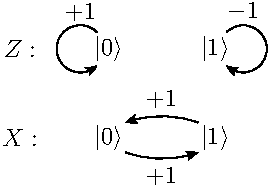
\includegraphics[]{pic-zx.pdf}
\end{center}
From this picture we can see that $Z$ acts by \emph{stabilizing} the
state $\ket{0}$ and anti-stabilizing the $\ket{1}$ state.
The $Z$ operator has been reduced 
to two operators each acting on a one dimensional subspace:
$Z = +1 \oplus -1.$
The $X$ operator serves to ``bitflip'' the state between
these two subspaces.

But what happens if we get confused and end up swapping
the $X$ and $Z$ operators? We would like to see the $X$ operator
as stabilizing / anti-stabilizing two subspaces, together with the
$Z$ operator as bitflipping between these.
The trick is to consider the \emph{orbits} of the operator
we hope to act as a stabilizer.
In this case there is only one orbit, $\ket{0}+\ket{1}$
and indeed, the $Z$ operator bitflips this to another state
$\ket{0}-\ket{1}$ that is anti-stabilized by $X.$

We are going to be considering Hamiltonians built from
summing operators of this form.
In this paper we use a ``neg-Hamiltonian'' convention,
to save complicating expressions with negative signs.
The ground space corresponds to the \emph{largest} eigenvalue.

Building a Hamiltonian from a single $X$ or $Z$ term
we can find the ground space as the stabilized space
using orbits. Then the adjacent operator acts to bitflip
between the eigenspaces.
To further elucidate this idea we turn to another example.
Now we have a hamiltonian built from three commuting and
independent operators 
$$
    \Ham = XXI + IXX + ZZZ.
$$
Starting with $\ket{000}$ we compute the orbit state
as $\ket{000}+\ket{011}+\ket{110}+\ket{101}.$
This time we have three bitflip operators
one for each of the stabilizer operators:
$ZII, IIZ, IXI.$
(We could also have chosen $IZZ, ZZI, XXX.$)
For example, $ZII$ sends the ground state to
$\ket{000}+\ket{011}-\ket{110}-\ket{101}$
which is anti-stabilized by $XXI.$
The bitflip operators form an abelian group of
order $2^3 = 8$ and by appying each element of
this group to the ground state we get a basis
of our state space, which we call a \emph{symmetry
invariant basis.}

Now we consider a four qubit example:
$$
    \Ham = XXII + IIXX + ZIZI + IZIZ.
$$
This time the terms of the Hamiltonian do not form
an abelian group.
We will call the group generated by the terms in the Hamiltonian
the \emph{gauge} group, $G$.
The stabilizers in this case will be the elements of $G$
that commute with every other element in $G.$
By inspection we see these are generated by $\Stab_0=\{XXXX, ZZZZ\}.$
and we can choose the reduced gauge generators to be $R_0=\{XXII, ZIZI\}.$
The logical operators are generated by $L_0 = \{XIXI, ZZII\},$
and then the errors $T_0$ corresponding to $\Stab_0$ will
be $\{ZZZI, IIIX\}.$
All of this can be summarized in a table of anti-commuting pairs:
\begin{center}
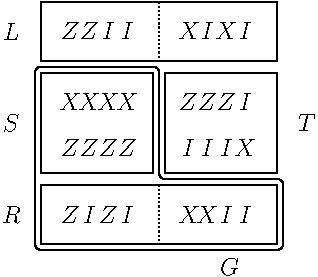
\includegraphics[]{pic-gauge4.pdf}
\end{center}
where the number of rows equals $n$ and each entry
commutes with the entries on other rows, and anticommutes
with the entry on the same row. 
If we take all the operators in the left column
we get the operators 
$\{ ZZII, XXXX, ZZZZ, ZIZI \}.$ 
These generate an abelian group 
that stabilizes the
state $\ket{\psi} = \ket{0000}+\ket{1111}.$
Let $r$ be the gauge operator $XXII$ adjacent to the 
stabilizer $ZIZI$,
The state $\ket{\psi}$ then lies in the $G-$orbit 
$$
\{\ket{\psi}, r\ket{\psi}\} = \{\ket{0000}+\ket{1111}, \ket{1100}+\ket{0011}\}.
$$
We use the $T_0$ operators $t_1=ZZZI$ and $t_2=IIIX$
to list three other $G-$orbits:
$$
\{t_1 \ket{\psi}, t_1 r\ket{\psi}\}, 
\{t_2 \ket{\psi}, t_2 r\ket{\psi}\}, 
\{t_1 t_2 \ket{\psi}, t_1 t_2 r\ket{\psi}\}.
$$
Here we have sixteen vectors forming an orthogonal basis for the state space.
They are arranged on the vertices of a cube. This cube is actually a four
dimensional hypercube, but we suppress the last dimension in
this diagram.
Such an arrangement of basis vectors has a cartesian product
structure which induces a tensor product decomposition of
the original state space.
\begin{center}
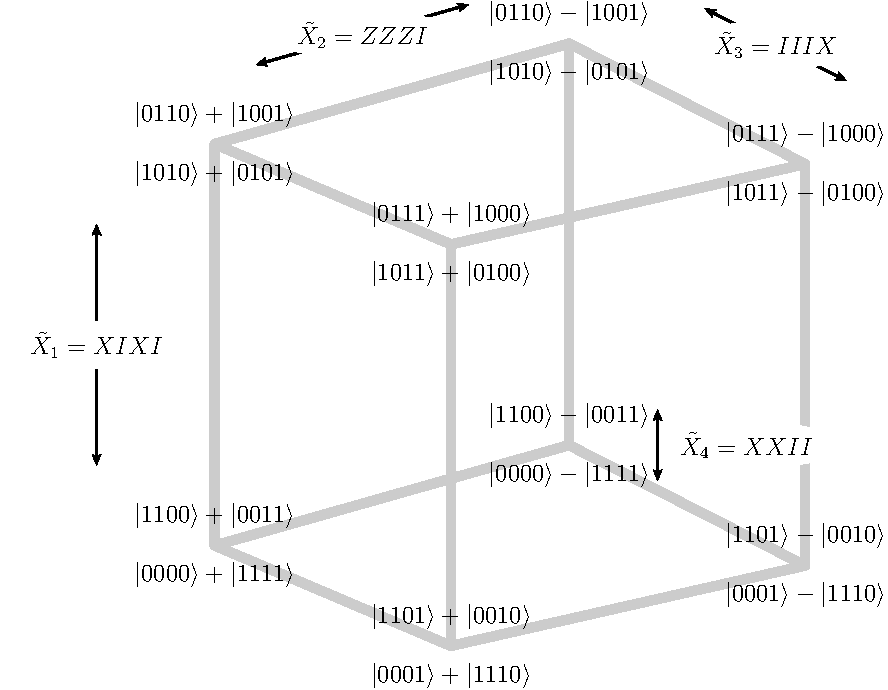
\includegraphics[width=0.7\columnwidth]{pic-operators.pdf}
\end{center}
The Hamiltonian acts on states by left multiplication.
Because this action
is a sum of gauge group elements,
it will decompose into blocks,
one for each $G-$orbit.
We depict this action as a weighted graph, where we omit edges
with zero weight:
\begin{center}
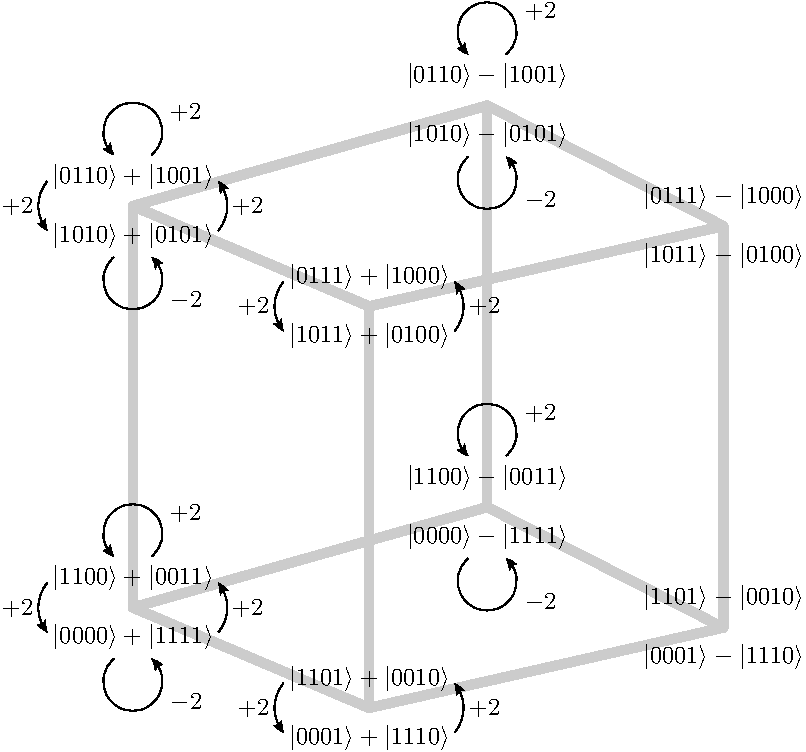
\includegraphics[width=0.7\columnwidth]{pic-orbit.pdf}
\end{center}

\def\Xt{\tilde{X}}
\def\Zt{\tilde{Z}}

\begin{align*}
\Ham &= XXII + IIXX + ZIZI + IZIZ \\
  &= \Xt_4 + \Zt_2\Xt_4 + \Zt_4 + \Zt_3\Zt_4 \\
  &= (I+\Zt_2)\Xt_4 + (I+\Zt_3) \Zt_4.
\end{align*}

Using the symmetry invariant basis computed from the orbits we
can write the matrix for the Hamiltonian in
block diagonal form:
$$
\Ham = 
\left( \begin{array}{cccc}
2(X+Z) & 0 & 0 & 0 \\
0  & 2X & 0 & 0 \\
0  & 0 & 2Z & 0 \\
0  & 0 & 0 & 0 \\
\end{array} \right) \otimes I
$$



\subsection{Complex representations}

\subsubsection{The Pauli group}

The Pauli group $\Pauli_1$ is normally 
defined as a set of matrices closed under
matrix multiplication, but we can define
it abstractly
as the group generated
by the (abstract) elements $\{\omega, X, Z\}$ with
relations as follows:
$$
\omega^2=I,\ X^2=I,\ Z^2=I,\ \omega X\omega X=I,\ \omega Z\omega Z=I,\ \mbox{and}\  \omega ZXZX=I,
$$
where $I$ is the group idenity.
Actually, $\omega $ is generated by $X$ and $Z$, so
it is not necessary to include $\omega $ in the generating set,
but here it simplifies the relations.
\footnote{We leave out $Y$ because...}
This group has eight elements, and is isomorphic to the dihedral group $D_4$,
the symmetry group of a square.

To define
the {\it $n$-qubit Pauli group} $\Pauli_n$, 
we use the $2n+1$ element 
generating set 
$$\{\omega , X_1, .., X_n, Z_1, .., Z_n\}$$
with relation $\omega^2=I$ as before, and
\begin{equation}\label{presentation}
\begin{array}{c}
X_i^2=I,\ Z_i^2=I,\ \omega X_i\omega X_i=I,\ \omega Z_i\omega Z_i=I,\ \omega Z_iX_iZ_iX_i=I, 
\mbox{\ for\ } i=1,...n,\\
Z_iX_jZ_iX_j=I, \mbox{\ for\ } i, j = 1,..,n,\ i\ne j.
\end{array}
\end{equation}

This abstract approach to the definition of a group is known as
a group {\it presentation}. In general, this is a set of
generators together with a set of relations satisfied
by these generators.

Note that each of the generators squares to the identity,
and of these, only $\omega$ commutes with every element of $\Pauli_n.$
%Note that $\omega$ commutes with all elements of $\Pauli_n$
%and squares to the idenity, 
Therefore we will write $\omega$ as $-I,$
similarly $\pm I$ will denote the
set $\{\omega, I\},$ and $-X$ is $\omega X$, etc.

We write the group commutator as
$[[g, h]]:=ghg^{-1}h^{-1}$
and note the important commutation relation:
$$
    [[Z_i, X_j]] = 
    \left\{ \begin{array}{ll}
 -I &\mbox{if}\ i=j,\\
 I &\mbox{if}\ i\ne j.\end{array}\right.
$$
If we take an arbitrary $g\in \Pauli_n$
written as a product of the generators,
it follows that we can rewrite this
product uniquely as %in an ordered fashion:
$ g = \pm g_1 ... g_n $
where each $g_i$ is one of $I, Z_i, X_i$ or $X_i Z_i$
for $i=1,..,n.$
Therefore, the size of the
Pauli group is 
$$
    |\Pauli_n| = 2^{2n+1}.
$$

%Elements of $\Pauli_n$ that consist of
%products of only $I$ or $X$ will
%be call $X$-type elements (or operators)
%and similarly $Z$-type elements are 
%products of only $I$ or $Z$.
The subgroup of $\Pauli_n$ generated by
the elements $\{X_1,...,X_n\}$ % $\{X_i\}_{i=1,..,n}$ 
is denoted $\Pauli_n^X.$ These are the $X$-type
elements. Similarly,
 $\{Z_1,...,Z_n\}$ generates % $\{Z_i\}_{i=1,..,n}$ 
the subgroup of $Z$-type elements $\Pauli_n^Z$.

\subsubsection{Subgroups of the Pauli group}

We now define an {\it $n-$qubit gauge group} to be 
any non-abelian subgroup $G$ of $\Pauli_n,$
defined by a set of generators $G_0\subset \Pauli_n,$
%for some subgroup $G$ of $\Pauli_n:$
$$ G := \langle G_0\rangle.$$
%We will assume $G$ is not abelian, which 
%%is equivalent to the condition that $-I\in G.$ % No! {-I, I} is abelian...
%implies that $-I\in G.$
Because $G$ is not abelian, it follows that $-I\in G.$
We also restrict $G_0$ to only contain Hermitian operators,
which is equivalent to requiring that $g^2=I$ for all $g\in G_0.$

Now let $\Stab$ be the largest subgroup of $G$ not containing
$-I.$
$\Stab$ is then an abelian subgroup,
also known as the {\it stabilizer} subgroup.
%(Note that each of the stabilizers commutes with the Hamiltonian.)
$G$ decomposes as a direct product:
$$G = \Stab\times R,$$
where $R\cong P_r$ for some $1\le r\le n,$
and $\Stab\cong \Z_2^{m}$ for $0\le m<n.$
Therefore, 
$$|G| = |\Stab| |R| = 2^{m+2r+1}.$$
We call $R$ the {\it reduced gauge group}.
We consider both $\Stab$ and $R$ to be subgroups of $G.$
%Let $\phi:P_r\to R$ be a group isomorphism,
Let $\phi:R\to P_r$ be a group isomorphism,
%then $R_0 := \{\phi(X_i), \phi(Z_i)\}_{1\le i\le r}$
%then $R_0 := \{\phi(X_i), \phi(Z_i)\}_{i=1,..,r}$
then $R_0 := \{\phi^{-1}(X_i), \phi^{-1}(Z_i)\}_{i=1,..,r}$
is a set of independent generators of $R.$
We also let $\Stab_0$ be a set of $m$ independent generators of $\Stab.$

To find the cosets of $G$ in $\Pauli_n$ we take
the group closure of $G-\Pauli_n$; when this is non-empty
we only need to add $I$ and $-I.$
This is another
gauge group, whose reduced gauge group is known as
the {\it logical} operators $L$, and whose 
stabilizer subgroup is known as the {\it error} operators $T.$
Now any coset of $G$ can be written as $ltG$ with
$l\in L$ and $t\in T.$
The size of $T$ equals the size of $\Stab$: $|T|=|\Stab|=2^m.$
If we let $L_0$ be an independent generating set for $L$
then we have the important formula:
\begin{align}
n &= \frac{1}{2}|L_0| + |\Stab_0| + \frac{1}{2}|R_0|\\
  &= k + m + r
\end{align}
We summarize the information in this section in a table
of Pauli group elements arranged in
two columns and $n$ rows:
\begin{center}
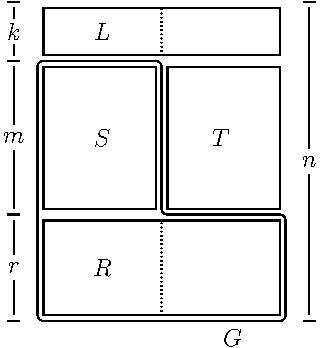
\includegraphics[]{pic-canonical.pdf}
\end{center}
Here we show the $2n$ generators of $\Pauli_n$ arranged 
so that each row contains a pair of generators,
where each such generator anti-commutes with the operator on the same row and
commutes with all the other operators in the table.
Note that this is exactly the definition of the Pauli group
via a presentation given in the previous section.
Furthermore, the table shows $2k$ generators
of $L$, $m$ generators each for $S$ and $T,$ and $2r$
generators of $R.$
The gauge group $G$ encloses $R$ and $S$, and one can
immediately see how $L$ and $T$ also form a gauge group.


\subsubsection{Representations of the Pauli group}

We now define the
{\it Pauli representation} 
of the Pauli group as a group homomorphism:
$$
    \rho_{\mathrm{pauli}} : \Pauli_n \to \GL(\Complex[2^n])
$$
where $\Complex[2^n]$ is the $2^n$-dimensional state space of $n$ qubits.
On the independent generators 
$\{X_1, .., X_n, Z_1, .., Z_n\},\ \rho_{\mathrm{pauli}}$
is defined as the following tensor product of $2\times 2$ matrices:

%$$
%\rho_{\mathrm{pauli}}(X_i) := \bigotimes_{j=1}^n \left\{ \begin{array}{ll}
%\left( \begin{array}{ll}
%1&0\\
%0&1\end{array} \right) &\mbox{for $j\ne i$,}\\
%\\
%\left( \begin{array}{ll}
%0&1\\
%1&0\end{array} \right) &\mbox{for $j=i$} \end{array}
%\right\},\ 
%\rho_{\mathrm{pauli}}(Z_i) := \bigotimes_{j=1}^n \left\{ \begin{array}{ll}
%\left( \begin{array}{ll}
%1&0\\
%0&1\end{array} \right) &\mbox{for $j\ne i$,}\\
%\\
%\left( \begin{array}{rr}
%1&0\\
%0&-1\end{array} \right) &\mbox{for $j=i$}\end{array}
%\right\}.
%$$

\begin{align*}
\rho_{\mathrm{pauli}}(X_i) := &\bigotimes_{j=1}^n \left\{ \begin{array}{ll}
\left( \begin{array}{ll}
0&1\\
1&0\end{array} \right) &\mbox{for $j=i$}\\
\\
\left( \begin{array}{ll}
1&0\\
0&1\end{array} \right) &\mbox{for $j\ne i$} \end{array}
\right.\\
\rho_{\mathrm{pauli}}(Z_i) := &\bigotimes_{j=1}^n \left\{ \begin{array}{ll}
\left( \begin{array}{ll}
1&0\\
0&-1\end{array} \right) &\mbox{for $j=i$}\\
\\
\left( \begin{array}{rr}
1&0\\
0&1\end{array} \right) &\mbox{for $j\ne i$}\end{array}
\right.
\end{align*}

%on $n$ qubits, $\Pauli_n,$
%as the set of $n$-fold tensor products
%of the matrices $\pm I, X, Z:$
%$$
%I = \left( \begin{array}{ll}
%1&0\\
%0&1\end{array} \right),\quad
%X = \left( \begin{array}{ll}
%0&1\\
%1&0\end{array} \right),\quad
%Z = \left( \begin{array}{ll}
%1&0\\
%0&-1\end{array} \right).
%$$

Normally the image of 
$\rho_{\mathrm{pauli}}$ is thought of as the
Pauli group itself, and we are indeed free to think
that way because $\rho_{\mathrm{pauli}}$ is a group
isomorphism.

Given a group representation $\rho:G\to GL(V)$
the {\it character} of $\rho$ is a function
$\chi_\rho:G\to \Complex$ given by
$$
    \chi_\rho(g) = \mbox{Tr}\ \rho(g).
$$

Given two functions $u,v : G \to \Complex$ 
we define the following inner product:
$$
    \langle u, v \rangle := \frac{1}{|G|} \sum_{g\in G} u(g) \overline{v(g)}.
$$

The character of the Pauli representation, $\chi_{{pauli}}:\Pauli_n\to\Complex$
is given by:
$$
\chi_{{pauli}}(g) = \sum_{v \in basis} \langle v | \rho_{{pauli}}(g) | v \rangle
    = \left\{ \begin{array}{ll}
 \pm 2^n &\mbox{if}\ g=\pm I\\
 0 &\mbox{otherwise}\end{array}\right.
$$

Since $|P_n|=2^{2n+1}$ it follows that
$\langle\chi_{pauli},\chi_{pauli}\rangle = 1$ and
so $\rho_{pauli}$ is an irreducible representation of $\Pauli_n.$

%It turns out %(see Appendix for details)
%that $\rho_{\mathrm{pauli}}$ is an
%irreducible representation ({\it irrep}) of $\Pauli_n$. 
The only other irreps of $\Pauli_n$ are 
the $1$-dimensional irreps $\rho:\Pauli_n\to\Complex$
defined on the independent generators as:
    $$ \rho(X_i) = \pm 1,\quad \rho(Z_i) = \pm 1.$$

So we have $2^{2n}$ many $1$-dimensional irreps,
and a single $2^n$-dimensional irrep.
Summing the squares of the dimensions
shows that we have a complete set of irreps of $\Pauli_n.$

%\subsubsection{Representations of stabilizer groups}
%
%Any abelian subgroup $\Stab\subset \Pauli_n$
%that does not contain $-I$ we call a stabilizer group.
%The reason for this name is...


\subsubsection{Representations of gauge groups}

%Our next job will be to find the irreps of {\it subgroups} of $\Pauli_n.$
Although $\rho_{\mathrm{pauli}}$
restricted to a gauge group $G\subset\Pauli_n$ serves as a representation
of $G$ it is no longer irreducible.
Our aim will be to decompose $\rho_{\mathrm{pauli}}$ into irreps of $G.$

The $1$-dimensional irreps $\rho:G\to \Complex,$
are now defined by
specifying the action of $\rho$ on the independent generators:
$$
    \rho(h)=\pm 1\ \mbox{for}\ h\in \Stab_0,
    \quad \rho(\phi^{-1}(X_i)) = \pm 1,\quad \rho(\phi^{-1}(Z_i)) = \pm 1.
$$
This gives all $2^{m+2r}$ of the $1$-dimensional irreps.
%These will turn out not to be used below.

The $2^r$-dimensional irreps are given by:
$$
    \rho(h) = \pm I^{\otimes r}\ \mbox{for}\ h\in \Stab_0,
    \quad \rho(\phi^{-1}(X_i)) = X_i,\quad \rho(\phi^{-1}(Z_i)) = Z_i.
$$
We are free to choose the signs of the $\rho(h)$ for each $h\in \Stab_0.$
Hence there are $2^m$ many of these irreps.
Each such choice corresponds to the choice of a {\it syndrome} vector $s(h)=\pm 1$, for $h \in \Stab_0,$
or alternatively, choice of an element $t\in T:$
$$
    \rho^1_t(h) = \left\{ \begin{array}{ll}
 I^{\otimes r}\ &\mbox{if $th=ht$}\\
 -I^{\otimes r}\ &\mbox{if $th=-ht$}\end{array} \right. %\right\}\mbox{for}\ h\in \Stab_0.
$$

%Finally, there are $2^m$ many $2^r$-dimensional irreps $\rho_t$
%which are labelled by $t\in T$ and defined as
%$$
%    %\rho_t(h)=\pm I^{\otimes 2^r}\ \mbox{for}\ h\in \Stab_0,
%    %\rho_t(h)= [t,h] = th^{-1}th^{-1} = \pm I^{\otimes 2^r}\ \mbox{for}\ h\in \Stab_0,
%    \rho_t(h) = \left\{ \begin{array}{ll}
% I^{\otimes 2^r}\ &\mbox{if $th=ht$}\\
% -I^{\otimes 2^r}\ &\mbox{if $th=-ht$}\end{array} \right\}\mbox{for}\ h\in \Stab_0,
%    \quad \rho_t(\phi^{-1}(X_i)) = X_i,\quad \rho_t(\phi^{-1}(Z_i)) = Z_i.
%$$

%For $G$ a subgroup of $\Pauli_n$, and decomposition
Because $G$ decomposes 
into a direct product $G=\Stab\times \Pauli_r$ we have the
following representations:
$$
    \rho_t(g) = \rho^1_t(h) \rho^r_{pauli}(g'),
$$
where $g=hg'$, $h\in \Stab$, $g'\in \Pauli_r$ 
%and $\rho_1(h)$ is a $1$-dimensional representation of $\Stab$.
and $\rho^r_{pauli}$ is the $r$-qubit Pauli representation.
The character for this representation is:
$$
\chi_{t}(hg') = \rho_t^1(h) \sum_{v \in basis} \langle v | \rho^r_{{pauli}}(g') | v \rangle
    = \left\{ \begin{array}{ll}
 \pm 2^r\rho_t^1(h) &\mbox{if}\ g'=\pm I\\
 0 &\mbox{otherwise}\end{array}\right.
$$

We have that $|G|=2^{2r+m+1}$ and so
$\langle\chi_{t},\chi_{t}\rangle = 1$ and
$\rho_t$ is an irreducible representation of $G.$
We now count the occurances of 
this representation in $\rho^r_{pauli}$:
\begin{align*}
\langle\chi^r_{pauli},\chi_{t}\rangle &= \frac{1}{|G|}\sum_{g\in G} \chi^r_{pauli}(g)\overline{\chi_{t}(g)} \\
&= \frac{1}{2^{2r+m+1}} \sum_{g=\pm I} 2^n 2^r = \frac{2^{n+1+r}}{2^{2r+m+1}} = 2^k
\end{align*}
where $k$ is the number of logical qubits so that $n=r+m+k.$

%\noindent{\bf Theorem.}
%Using characters one can show that
%on a subgroup $G$ of $\Pauli_n$ the
In summary, the Pauli representation decomposes into 
$2^m$ many irreps $\rho_t,$ 
each with dimension $2^r,$ 
and appearing with multiplicity $2^k:$
$$
    \rho_{\mathrm{pauli}} = 
        \bigoplus_{t\in T}\ \rho_t \otimes I^{\otimes k}
$$
%where we label the $2^r$-dimensional irreps by $t\in T.$
%See appendix for details.

\subsubsection{Symmetry invariant basis}

In general, given a representation $\rho:G\to \GL(V)$
and the character of some irreducible representation $\chi:G\to \C$
the following operator 
$P:V\to V$
projects onto the subspace on which
this irreducible representation acts:
$$
    P := \frac{d}{|G|} \sum_{g\in G} {\overline{\chi(g)}} \rho(g).
$$
where $d$ is the dimension of the irreducible representation.
We can use this to calculate projectors onto the irreps $\rho_t$ in $\rho_{pauli}$:
\begin{align*}
P_t &= \frac{d}{|G|} \sum_{g\in G} \overline{\chi_t(g)} \rho_{pauli}(g) \\
    &= \frac{d}{|G|} \sum_{h\in \Stab}\sum_{g\in R} \overline{\chi_t(hg)} \rho_{pauli}(hg) \\
    &= \frac{d}{|G|} 2^{2r} \sum_{h\in \Stab} {\rho^1_t(h)} \rho_{pauli}(h) \\
    &= \frac{1}{2^m} \sum_{h\in \Stab} {\rho^1_t(h)} \rho_{pauli}(h).
\end{align*}

We can also write this as a product of projectors onto
the $\pm 1$ eigenspaces of stabilizers $\rho_{pauli}(h)$ for $h\in \Stab.$
Choose generators $h_1,...,h_m$ of $S$
and then the projectors onto the $\pm 1$ eigenspace of $\rho_{pauli}(h_i)$ are
$$
P^i_t = \frac{1}{2} \bigl(I^{\otimes n} \pm \rho_{pauli}(h_i) \bigr)
$$
and we see that 
$$
P_t = \prod_{i=1,...,m} P^i_t 
    = \frac{1}{2^m} \bigl(I^{\otimes n} \pm \rho_{pauli}(h_1)\bigr)
    ...\bigl(I^{\otimes n} \pm \rho_{pauli}(h_m)\bigr).
$$
This projector will have rank $2^{k+r}$ and
$$
U := \sum_{t\in T} P_t
$$
is a unitary transformation that sends
physical qubits to encoded qubits.


\subsection{The Hamiltonian}

The Hamiltonian of interest is 
an operator $\Ham:\Complex[2^n]\to\Complex[2^n]$:
%and normally defined
%as the negative sum of terms from $G_0,$ but here
%we will reverse the sign:
$$ \Ham := \sum_{g\in G_0} \rho_{\mathrm{pauli}}(g).$$
Using the above decomposition we find:
\begin{align*}
    \Ham &= \sum_{g\in G_0}\ \bigoplus_{l\in L, t\in T}\ \rho_t(g)\\
         &= \bigoplus_{l\in L, t\in T} \sum_{g\in G_0}\ \rho_t(g).
\end{align*}
%The goal is to decompose $\Ham$ into blocks as
%$$
%    \Ham = \bigoplus_{\mathrm{irrep}\rho} \sum_{g\in G_0}\ \rho(g),
%$$
We will notate each block as
$\Ham_t := \sum_{g\in G_0}\rho_t(g)$
for each irrep $\rho_t$ appearing in $\Ham.$
\begin{framed}
\noindent{\bf Fact 0:}

The Hamiltonian is block diagonalized, with blocks indexed by operators $t$ in
the abelian group $T$ and multiplicity $2^k:$
$$
    \Ham =  \bigoplus_{t\in T}\ \Ham_t \otimes I^{\otimes k}.
$$
\end{framed}
%Writing $I$ for the identity element of $T$ we write the corresponding
%block of the hamiltonian as $\Ham_{0,0}.$

More generally, we can assign real valued weights
$J_g\in\R$
to each operator $g\in G_0,$
\begin{align*}
    \Ham = \sum_{g\in G_0} J_g \rho_{\mathrm{pauli}}(g)
            = \bigoplus_{l\in L, t\in T} \sum_{g\in G_0}\ J_g \rho_t(g).
\end{align*}
In other words, using weights does not change the block structure of $\Ham.$

%%%%%%%%%%%%%%%%%%%%%%%%%%%%%%%%%%%%%%%%%%%%%%%%%%%%%%%%%%%%%%%%%%%%%%%%%%%%%%%
%
%%%%%%%%%%%%%%%%%%%%%%%%%%%%%%%%%%%%%%%%%%%%%%%%%%%%%%%%%%%%%%%%%%%%%%%%%%%%%%%
%

\subsection{Applications}

In the following applications we will make the identification
between $g$ and $\rho_{pauli}(g)$.
So terms such as $Z$ and $X$ are understood
to be the corresponding Pauli linear operators.

%%%%%%%%%%%%%%%%%%%%%%%%%%%%%%%%%%%%%%%%%%%%%%%%%%%%%%%%%%%%%%%%%%%%%%%%%%%%%%%
%
%%%%%%%%%%%%%%%%%%%%%%%%%%%%%%%%%%%%%%%%%%%%%%%%%%%%%%%%%%%%%%%%%%%%%%%%%%%%%%%
%

\subsubsection{2D compass model}

Here we consider the two-dimensional compass model \cite{Bacon2006}.
We coordinatize the qubits on a square 
lattice of\ $l\times l$\ sites,
$(i, j)$\ for\ $1\le i, j\le l.$
This gives $n = l^2.$
For the single qubit Pauli operators acting on site
$(i, j)$ we coordinatize with subscripts $ij$, 
with $i$ and $j$ understood modulo $l$.
The generators of the gauge group are
$$
    G_0 = \big\{ X_{ij}X_{i,j+1},\ Z_{ij}Z_{i+1,j}\ \mbox{for}\ 1\le i, j\le l\big\}.
$$
We write generators of the reduced
gauge group in anti-commuting pairs:
$$
    R_0 = \big\{ X_{i1}X_{ij},\ Z_{1j}Z_{ij}\ \mbox{for}\ 2\le i, j\le l\big\}.
$$
This makes it clear the isomorphism $\phi : R \to \Pauli_r$ to use,
and we again use pairs $i,j$ to coordinatize $\Pauli_r$:
$$
    \phi(X_{i1}X_{ij}) = X_{i-1,j-1}, \ \ \phi(Z_{1j}Z_{ij}) = Z_{i-1,j-1},\ \mbox{for}\ 2\le i, j\le l.
$$
The generators for the stabilizers are
$$
    \Stab_0 = \big\{ \prod_{i=1}^l X_{ij}X_{i,j+1},\ \prod_{i=1}^l Z_{ji}Z_{j+1,i}\ \mbox{for}\ 1\le j\le l-1\big\}.
$$
The logical operators are generated by $L_0 = \big\{ \prod_i X_{i1}, \prod_j Z_{1j} \}.$
These sets have cardinalities:
$$|G_0|=2l^2,\ |R_0| = 2(l-1)^2,\ |\Stab_0| = 2(l-1).$$
%And we note that $\frac{1}{2}|L_0| + |\Stab_0| + \frac{1}{2}|R_0| = n.$
And we note that $k+m+r=n$ is satisfied.
%Now we can define the irreps of $G$.
Now we write down the values of the
irreps on the gauge operators.
Here we define each irrep using a pair 
of syndrome vectors $s_X$ and $s_Z:$
\begin{align*}
\rho(X_{i1} X_{i2}) &= X_{i-1,1} &
%\rho(Z_{1i} Z_{2i}) &= Z_{1,i-1} &\mbox{for}\ 2\le i\le l\\
\rho(Z_{1i} Z_{2i}) &= Z_{1,i-1} \\&&&\mbox{for}\ 2\le i\le l\\
\rho(X_{il} X_{i1}) &= X_{i-1,l-1} &
%\rho(Z_{li} Z_{1i}) &= Z_{l-1,i-1} &\mbox{for}\ 2\le i\le l\\
\rho(Z_{li} Z_{1i}) &= Z_{l-1,i-1} \\&&&\mbox{for}\ 2\le i\le l\\
\rho(X_{ij} X_{i,j+1}) &= X_{i-1,j-1} X_{i-1,j} &
%\rho(Z_{ji} Z_{j,i+1}) &= Z_{j-1,i-1}Z_{j,i-1} &\mbox{for}\ 2\le i\le l, 2\le j<l\\
\rho(Z_{ji} Z_{j,i+1}) &= Z_{j-1,i-1}Z_{j,i-1} \\&&&\mbox{for}\ 2\le i\le l, 2\le j<l\\
\rho(X_{1j} X_{1,j+1}) &= s_X(j-1) \prod_{i=1}^{l-1} X_{i,j-1} X_{ij} &
%\rho(Z_{j1} Z_{j+1,1}) &= s_Z(j-1) \prod_{i=1}^{l-1} Z_{j-1,i} Z_{ji} &\mbox{for}\ 2\le j<l\\
\rho(Z_{j1} Z_{j+1,1}) &= s_Z(j-1) \prod_{i=1}^{l-1} Z_{j-1,i} Z_{ji} \\&&&\mbox{for}\ 2\le j<l\\
\rho(X_{11} X_{12}) &= \prod_{j=1}^{l-1}s_X(j) \prod_{i=1}^{l-1} X_{i1} &
\rho(Z_{11} Z_{21}) &= \prod_{j=1}^{l-1}s_Z(j) \prod_{i=1}^{l-1} Z_{1i}.
\end{align*}
Note the transposition symmetry between the $X$ and $Z$-type operators.
We sum all these terms to find 
the form of the hamiltonian in each block:
$$
\Ham_\rho = \sum_{g\in G_0} \rho(g) = \sum_{1\le i,j<l} \rho(X_{ij}X_{i,j+1}) + \rho(Z_{ij}Z_{i+1,j}).
$$
We note that in \cite{Brzezicki2013},
they perform a
spin transformation of the compass model
which also results in an $(l-1)\times(l-1)$ lattice
of spins and identical Hamiltonian up to some signs.

Note that the form of each of the Hamiltonian blocks $H_t$
comes from another gauge code.
In this case it has some non-local operators, as well as $\pm 1$ factors
which can be subsumed into the gauge code as operators $\pm I.$

%We have the following important fact which we will prove in section \ref{spectra} below:
%\begin{framed}
%\noindent{\bf Fact 1:}
%
%The blocks $H_t$ of a CSS gauge code Hamiltonian are also CSS.
%\end{framed}
%
%By counting dimensions we can conclude the following:
%\begin{framed}
%\noindent{\bf Fact 2:}
%
%Each block $H_t$ has non-degenerate groundspace.
%\end{framed}
%
%\emph{!! check what happens with weights $\pm 1.$}

%\fbox{\parbox[b]{5cm}{This is long text that will be wrapped once it reaches five centimeters.}}

%%%%%%%%%%%%%%%%%%%%%%%%%%%%%%%%%%%%%%%%%%%%%%%%%%%%%%%%%%%%%%%%%%%%%%%%%%%%%%%
%

\subsubsection{The $XY$-model}

The $XY$-model lives on a one dimensional chain of $n$ qubits.
We write the gauge group generators as
$$
    G_0 = \{ X_i X_{i+1}, Z_i Z_{i+1} \ \mbox{for}\ i=1,...,n \}
$$
with periodic boundary conditions.

This example shares features of both the previous and the next examples.



%%%%%%%%%%%%%%%%%%%%%%%%%%%%%%%%%%%%%%%%%%%%%%%%%%%%%%%%%%%%%%%%%%%%%%%%%%%%%%%
%

\subsubsection{Kitaev honeycomb model}


%\begin{figure*}[th!]
%\begin{center}
%        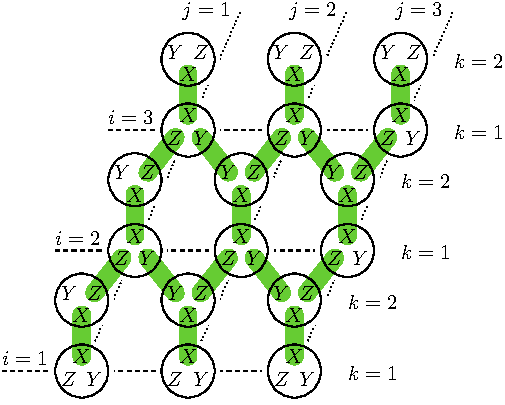
\includegraphics[width=0.6\columnwidth]{fig_00.pdf}
%\caption{
%Gauge generators have support on the edges of the honeycomb lattice.
%Qubits here are depicted as circles.
%}
%\label{honeycomb}
%\end{center}
%\end{figure*}


The Kitaev honeycomb model \cite{Kitaev2006} is built from spins on
the sites of a hexagonal lattice. 
The lattice of linear size $l$ has $n=2l^2$ sites
which we coordinatize using integer triples $i, j, k$
with $1\le j, k\le l$ and $k=1, 2.$
We use periodic boundary conditions so $i, j$ are
to be taken modulo $l$.
Gauge generators have support on the edges of the honeycomb lattice,
and we depict qubits here as circles:
\begin{center}
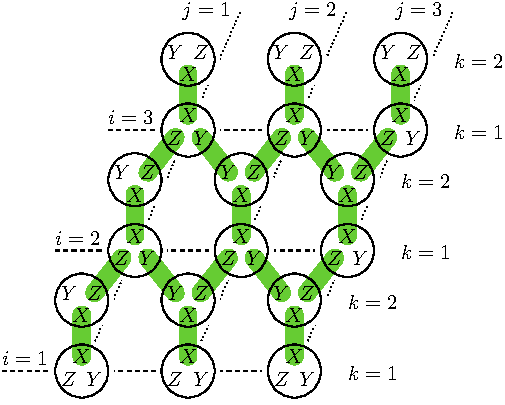
\includegraphics[width=0.6\columnwidth]{fig_00.pdf}
\end{center}
%See figure \ref{honeycomb}.
The edges of the lattice are in one-to-one
correspondence with the generators $G_0$:
$$
G_0 := \big\{X_{ij1}X_{ij2},\ Z_{ij2}Z_{i+1,j1},\ Y_{ij1}Y_{i-1,j+1,2}
\ \mbox{for}\ 1\le i,j\le l\big\}.
$$
Note that we make the definition $Y:=XZ$ for each site.

Stabilizers are generated from closed strings of
gauge operators. 
For example, each hexagon gives a stabilizer
\begin{align*}
h_{ij}:&= 
X_{ij1}X_{ij2}
Z_{ij2}Z_{i+1,j1}
Y_{i+1,j1}Y_{i,j+1,2}
X_{i,j+1,2}X_{i,j+1,1}
Z_{i,j+1,1}Z_{i-1,j+1,2}
Y_{i-1,j+1,2}Y_{ij1}
\\
&= 
Z_{ij1} Y_{ij2} X_{i+1,j1}
Z_{i,j+1,2} Y_{i,j+1,1} X_{i-1,j+1,2}.
\end{align*}

And the two homologically non-trivial loops
give stabilizers:
$$
h_v := \prod_{i=1}^l Y_{i11} Y_{i12},\ \ 
h_h := \prod_{j=1}^l X_{1j2} X_{2j1}.
$$

This gives independent stabilizer generators $\Stab_0$
from each hexagon, less one, as well as $h_v$ and $h_h.$
%two homologically non-trivial loops.
The number of hexagons is $\frac{1}{2}n$ and
so we find $|\Stab_0|=\half n+1.$
There are no logical operators, so we
must have $|R_0|=n-2.$

%\begin{figure*}[th!]
%\begin{center}
%        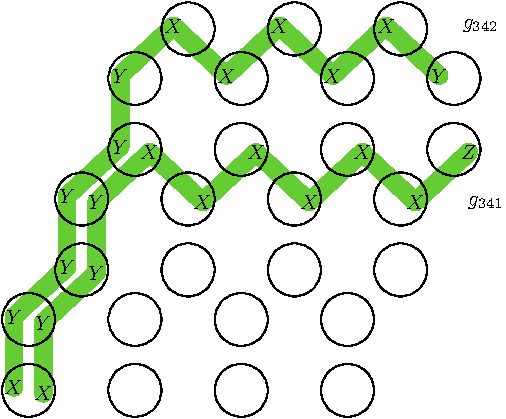
\includegraphics[width=0.5\columnwidth]{fig_01.pdf}
%%\caption{Two elements $g_{341}$ and $g_{342}$ of the set $R_0$}
%\caption{Two elements of the set $R_0$ corresponding
%to $i=3$, $j=4$ and $k=1,2.$}
%\label{jaws}
%\end{center}
%\end{figure*}

Now we construct a set of string operators $R_0$,
one for each site on the lattice, except for
the two sites $(1,1,1)$ and $(1,1,2).$
Each string $g_{ijk}\in R_0$
is constructed as the product of
gauge operators along a path starting at
$(1,1,1)$ and terminating at $(i,j,k).$
%See figure \ref{jaws}.

Two elements of the set $R_0$ corresponding
to $i=3$, $j=4$ and $k=1,2.$
\begin{center}
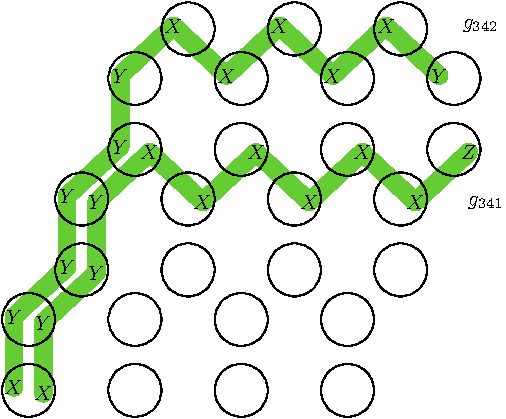
\includegraphics[width=0.5\columnwidth]{fig_01.pdf}
\end{center}

Each such path is built from two ``straight''
path segments, first in the $i$ direction
and then in the $j$ direction. 
The paths for operators $g_{ij1}$ and
$g_{ij2}$ coincide along the $i$ direction
but become disjoint in the $j$ direction:
the $g_{ij1}$ path goes around the bottom
of the hexagons and the $g_{ij2}$ path
goes around the top.
With periodic boundary conditions $R_0$ forms an
independent generating set of $R$ of size $n-2.$

We construct an isomorphism $\phi: R\to \Pauli_r$
by sending elements of $R_0$ bijectively
to the following independent generating
set of $\Pauli_r$:
$$
\big\{c_{2j}:=Z_1...Z_{j-1} X_j,\ c_{2j+1}:=Z_1...Z_{j-1} Y_j\ \ \mbox{for}\ 1\le j\le r\big\}.
$$
The bijection is constrained 
by setting $\phi(g_{ij1}):=c_{2j'+1}$
and $\phi(g_{ij2}):=c_{2j'}$
where $j'$ is chosen uniquely for each $i, j.$
The $c_j$ are paired Majorana fermion operators \cite{Kitaev2006}.

%We construct an isomorphism $\phi: R\to \Pauli_r$
%by setting $\phi(g_{ij1}):=c_{2j'}$
%and $\phi(g_{ij2}):=c_{2j'+1}$
%%we map 
%%elements of $R_0$ to the following independent generating
%where the $c_j$ form the following independent generating
%set of $\Pauli_r$:
%$$
%%\big\{\prod_{i=1}^{j-1} Z_i X_j,\ \prod_{i=1}^{j-1} Z_i Y_j\ \mbox{for}\ 1\le j\le r\big\}.
%\big\{c_{2j}:=Z_1...Z_{j-1} X_j,\ c_{2j+1}:=Z_1...Z_{j-1} Y_j\ \ \mbox{for}\ 1\le j\le r\big\}.
%$$

We check this is a group homomorphism by showing that relations
satisfied by elements of $R_0$ are satisfied by
their images under $\phi.$
All such relations are either of the form
$g^2=~\pm~I$, $gg'=\pm~g'g$, or
products thereof.
So it is sufficient to check squares of
elements and commutation relations.
Every element of $R_0$ anticommutes with
every other element of $R_0$, and this is true also
of the $c_j.$
Also, $g_{ij1}^2=-I$ and $g_{ij2}^2=I$ 
is preserved by $\phi$ because $c_{2j}^2=I$ and $c_{2j+1}^2=-I$.
Finally, $\phi$ is an isomorphism
because it is a bijection of two independent
generating sets.

The next step is to write each element of $G_0$
as a product of reduced gauge operators and stabilizers.
The key thing to note is that the product of two
operators $g_{ijk}, g_{i'j'k'}\in R_0$ gives a string
operator between the sites $(i,j,k)$ and $(i',j',k')$.
And {\it any} string operator between these
two sites can then be generated by using stabilizers to
``deform'' the string $g_{ijk}g_{i'j'k'}.$
For example, taking the product
of two operators from $R_0$ that differ
by one path segment gives the following:
\begin{align*}
Z_{ij2}Z_{i+1,j,1} &= g_{ij2} g_{i+1,j,1} \\
%&\mbox{for}\ \  1\le i<l,\ 1\le j\le l, \ \ \mbox{except}\ \  (i,j)=(1,1) \ \ \mbox{or}\ \ (l,1)\\
Y_{i+1,j,1}Y_{i,j+1,2} &= g_{i+1,j,1}g_{i,j+1,2}
%&\mbox{for}\ \  1\le i,j\le l, \ \ \mbox{except}\ \  (i,j)=(1,1) \ \ \mbox{or}\ \ (l,1).
\end{align*}
We need the homologically non-trivial stabilizers to get these:
\begin{align*}
Z_{lj2}Z_{1j1} &= h_v g_{lj2} g_{1j1} &\mbox{for}\ \  2\le j\le l
\end{align*}
And the $X_{ij1}X_{ij2}$
gauge operators can be generated
by the product of 
$g_{ij1}g_{ij2}$ and the enclosed hexagon stabilizers:
$$X_{ij1}X_{ij2}=g_{ij1}g_{ij2}\prod_{j'=1}^{j-1} h_{ij'}.$$

The only $G_0$ operators that are not 
quadratic in $R_0$ operators are the five
operators that touch either of the sites
$(1,1,1)$ or $(1,1,2)$.

So each block in the Hamiltonian
is seen to be quadratic in the $c_j$ plus
five other Pauli operator terms which we denote as $\Lambda_\rho$:
$$
    \Ham_\rho = \sum_{ij} \Gamma_{ij}(\rho) c_i c_j + \Lambda_\rho
$$
The coefficients $\Gamma_{ij}$ are dependant on the irrep $\rho.$

In \cite{Kells2009} they introduce a similar set of
mutually anti-commuting string operators $R_0.$

%A similar analysis applies to the ising model, Jordan-Wigner... 
%http://arxiv.org/pdf/1504.01444 page 86.

%%%%%%%%%%%%%%%%%%%%%%%%%%%%%%%%%%%%%%%%%%%%%%%%%%%%%%%%%%%%%%%%%%%%%%%%%%%%%%%
%

\def\Cn{\Complex[2^n]}
\def\Cr{\Complex[2^r]}
\def\Field{\mathcal{F}_2}
\def\Fn{\Field[n]}
\def\Fr{\Field[r]}

\subsection{Representations over the finite field $\Field$}

This is a way of ``brute-forcing'' the representations when
we cannot find a way of writing them down in a closed form expression.
For finite systems this yields an algorithm that is efficiently implementable.

In this section, and the remainder of this paper,
we restrict our
attention to gauge groups formed from terms 
in $\Pauli_n^X\cup\Pauli_n^Z.$
We call these \emph{CSS gauge codes.}
We briefly review the $\Field$ symplectic structure of
these operators.

Both $\Pauli^X_n$ and $\Pauli^Z_n$ are abelian groups,
and can be identified with the additive 
group structure of the $n$ dimensional vector space
over the finite field of two elements $\Field:$
$$
    \Pauli^X_n \cong \Fn,  \ \ 
    \Pauli^Z_n \cong \Fn. 
$$
we do this in the obvious way by sending $X_i$ to the basis vector with
$1$ in the $i-$th entry, and similarly for each $Z_i$. 
We also identify the computational basis of our statespace $\Complex[2^n]$
with $\Fn$ in the obvious way.
This has the potential to be very confusing but 
apart from $X$ and $Z$ subscripts
we resist the temptation to
use any other decorations.

$X$-type operators act on basis vectors using $\Field$ addition:
$$
    g_X \in \Pauli^X_n \cong \Fn, \ \ g_X : v \longmapsto g_X + v
$$

$Z$-type operators act on basis vectors using $\Field$ inner product:
$$
    g_Z \in \Pauli^Z_n \cong \Fn, \ \ g_Z : v \longmapsto g_Z v^\top
$$
This is an $\Field$ scalar, just zero or one. We think of this
as a ``syndrome''.
Our $\Field$ vectors come as row vectors by default,
so a product $u v^\top$ of
two $\Fn$ vectors is a scalar.

It doesn't make sense to add an $X$-type operator and
a $Z$-type operator:
$$
    g_Z + g_X \ \ \ \mbox{\emph{no no!!!}}
$$
but it does make sense to take the inner product:
$$
    g_Z g_X^\top = g_X g_Z^\top.
$$
This is an $\Field$ scalar which gives the commutator of the 
two operators.

We wish to use this language to decompose a CSS gauge group $G.$
First we write the gauge group generators in terms of
$X$-type and $Z$-type operators:
$$
    G_0 = G_X \cup G_Z.
$$
Following the theory from the previous section,
we are going to rewrite the gauge group generators
as a union of stabilizer generators $S_0 = S_X \cup S_Z$
and reduced gauge generators $R_0 = R_X \cup R_Z.$
Similarly, the error operators
will be split into $X$ and $Z$ type
operators $T_X$ and $T_Z$ and
finally the logical operators
$L_X$ and $L_Z.$

We summarize all of these sets
in the following table:
\def\Im{\mathrm{im}}
\def\Ker{\mathrm{ker}}
%\def\Span#1{\mathrm{span}(#1)}
\def\Span#1{\langle #1 \rangle}
\begin{center}
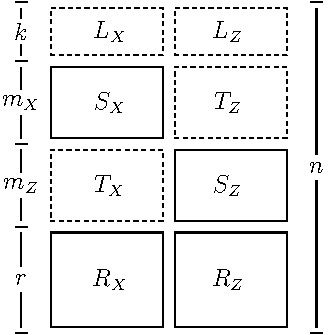
\includegraphics[]{pic-symplectic.pdf}
\end{center}

The solid rectangles indicate operators that
span the $X$ and $Z$ parts of the gauge group,
and the dashed rectangles indicate operators that
do not live inside the guage group.

We consider each of these blocks 
$L_X, L_Z, S_X, T_Z, T_X, S_Z, R_X, R_Z$
as either a set of $\Fn$ vectors or as an 
$\Field$-\emph{matrix}
with $n$ columns.
For example, we write $u\in R_X$ to mean $u$ is in
the set $R_X$. 
Given $v\in \Fr$ then $u = v R_X$ is
a generic vector in the rowspace of $R_X.$

We call the rowspace of an $\Field$-matrix
$M$ the \emph{span} and denote 
it as $\Span{M}.$
The kernel of $M$ is defined as
$$
    \Ker(M) = \{ v^\top | M v^\top = 0 \}.
$$

We first find the stabilizers $S_Z$.
These are built out of $\Fn$ vectors from the span of $G_Z$
that commute with the rows of $G_X:$
\begin{align*}
    \Span{S_Z} &= \{\  vG_Z \ |\  v G_Z G_X^\top = 0, \ \ v \in F_2^{|G_Z|}\ \} \\
               &= \{\  vG_Z \ |\  v^\top \in \Ker(G_X G_Z^\top)  \ \}.
\end{align*}
The generators (rows of $S_Z$) can be extracted
from the span by row reduction.
We swap the role of $X$ and $Z$ to find $S_X.$

Once we have the stabilizers, in order to
complete the above table as a presentation
of the Pauli group we need to solve the
following $\Field$ block matrix equation:
%All of this can be summarized in the block matrix equation:
$$
\left( \begin{array}{l}
L_X\\
S_X\\
T_X\\
R_X
\end{array} \right)
\left( \begin{array}{l}
L_Z\\
T_Z\\
S_Z\\
R_Z
\end{array} \right)^\top =
I.
$$
%And once again we have a presentation of the Pauli group.
with the restriction that the rows of
$R_X$ lie in the span of $G_X$ and
the rows of $L_X$ do not. Similarly
for $R_Z$ and $L_Z.$
This is a non-linear system of 16 equations and so it
is not obvious how to proceed, but it turns out a
systematic way can be found.

To find the reduced gauge group $R_X$ we project the gauge
group generators onto the orthogonal complement of $S_X.$
Such a projector is an $n\times n$
matrix given by
$$
    P_X = I + A^\top S_X
$$
where the matrix $A$ is the $m_X\times n$ matrix consisting of
the leading 1's in a row-reduction of $S_X.$
Then $R_X$ is found as a row-reduction of $G_X P_X.$
We find $R_Z$ in a similar way.

The logical operators $L_Z$ 
span the kernel of $G_X$ intersected with the complement
of the span of $H_Z.$

The error operators $T_X$ are found as the solution
to the linear system:
\begin{align*}
    H_Z T_X^\top &= I \\
    L_Z T_X^\top &= 0 \\
    R_Z T_X^\top &= 0
\end{align*}
\emph{and on it goes...}

We call this array of eight $\Field$
valued matrices 
an $(L,S,T,R)$-decomposition of the gauge group.
In general this will not be unique for
any given gauge group.

\subsubsection{The Hamiltonian}

The complex Hilbert state space of our
Hamiltonian has $2^n$ dimensions and we
write this space as $\Complex[2^n]$.
This notation is meant to suggest that
we are forming a $\Complex$ vector space
using $2^n$ ``points'' 
as basis vectors.
Working in the computational basis,
we do indeed have $2^n$ such points; 
these are the elements of $\Fn.$
And so we make the identification
$$
    \Complex[2^n] \cong \Complex[\Fn].
$$
In other words, we are labelling 
our basis vectors with elements of $\Fn$
and therefore such notation as
$$
    \bra{u} H \ket{v}
$$
with $u, v \in \Fn$ makes sense.
We will make further use of this below,
by writing computations in vector
spaces over $\Field$ inside the Dirac brakets.

Returning to the code $(L,S,T,R)$-decomposition
above,
given $t\in T$ such that $t = t_X t_Z$
we get a basis for the irrep $\rho_t$:
$$
    \{ \ket{v R_X + t_X} \ \mbox{such that}\  v \in \Fr \}.
$$
In other words,
the basis of the irrep $\rho_t$ is 
an affine subspace of $\Fn.$
Each such affine subspace is indexed by an
element of $\Fr$ and
all of these are
translates of each other,
so we make the following identification:
$$
\Complex[\{vR_X+t_X\}_{v\in\Fr}]
\cong \Complex[\Fr].
$$
This will allow us to write the components
of each block $H_t$ of the Hamiltonian
as $\bra{u}H_t\ket{v}$ for $u,v\in\Fr.$
We make this identification of affine subspaces
not out of laziness but because it will
help us to compare each of
the Hamiltonian blocks $H_t$ below.

\begin{framed}
\noindent{\bf Important:}
The computational basis identifies
basis vectors of $\Complex[2^n]$
with elements of a finite vector space $\Fn$:
$$
    \Complex[2^n] \cong \Complex[\Fn].
$$
The $(L,S,T,R)$-decomposition naturally
splits $\Fn$ into $2^{m_Z+k}$ affine subspaces:
$$
    \{ v R_X + t_X + l_X \}_{v\in\Fr}
$$
for each $t_X \in \Span{T_X}, l_X \in \Span{L_X}.$
Each such affine subspace forms a basis
for the irreducible blocks $H_{t_X,t_Z}$ of $H$,
and can be naturally identified with $\Fr:$
$$
    H_{t_X,t_Z} : \Complex[\Fr] \to \Complex[\Fr].
$$
\end{framed}

We now wish to understand the action of the
gauge group on each of its irreps.
Starting with the $t=0$ irrep,
this is where each of the stabilizers has
a trivial action. 
In $\Fn$ this
corresponds to additive action of the zero vector.

States $u\in\Span{R_X}$ can be built from a
vector matrix product
$$
    u = v R_X
$$
with $v\in\Fr.$
Since $R_X R_Z^\top = I$
we can write $v = u R_Z^\top.$
For each $g_X\in G_X$ these act as
\begin{align*}
    u_1 &= (u + g_X) \ \mbox{mod}\  S_X \\
        &= (u + g_X) P_X \\
        &= (v R_X + g_X) P_X.
\end{align*}
writing $u_1 = v_1 R_X$ we then have
\begin{align*}
    v_1 &= (v R_X + g_X) P_X R_Z^\top \\
        &= v + g_X P_X R_Z^\top.
\end{align*}

So we have that working in the computational
basis, the action of the $X$ part of the
gauge group in the $t=0,0$ irrep is to send
$v\in R_X$ to 
$v + g_X P_X R_Z^\top.$

%In the computational basis, the Hamiltonian
%is a $2^n\times 2^n$ element matrix which
%we can index using a pair of $\Fn$ vectors.
%Here we use a function notation for this:
%\begin{align*}
%    H : \Fn \times \Fn &\to \Complex
%        %(u, v) &\mapsto H(u, v).
%\end{align*}
%Each irrep of the gauge group 
%will then be acting on a subspace of 
%$\Cn$ spanned by basis vectors 
%
%$$
%    \Cn \cong \Complex[\Fn]
%$$

%Lets record this in our Hamiltonian block $H_{0,0}$
%by indexing the matrix components with a function notation. 
%The Hamiltonian takes a pair of
%basis vectors and produces a complex number:
%$H_{0,0} : \Fr\times\Fr \to \Complex.$

\newcommand{\pluseq}{\mathrel{+}=}

We have the following contributions from the
$G_X$ terms of the Hamiltonian:
$$
%    H_{0,0}(v, v+g_X P_X R_Z^\top) \ne 0,\ \ \mbox{for}\ g_X\in G_X, v\in \Fr
    \bra{v} H_{0,0} \ket{v+g_X P_X R_Z^\top} 
        \pluseq 1,\ \ \mbox{for}\ g_X\in G_X, v\in \Fr
$$
Where we use the $\pluseq$ notation
because there may be other ``contributions'' to the
same component.
These terms will always be off
the diagonal unless $g_X$ is a stabilizer.

The action of the $G_Z$ gauge group
contributes to the diagonal of $H.$
These diagonal terms apply a kind of
``potential energy'' penalty
to the basis states
that depends on the \emph{syndrome} vector:
$$
    \mbox{syndrome}(u) = G_Z u^\top
$$
for $u\in \Fn.$
This is an $\Field$ vector that has one component for
each row of $G_Z.$
Writing $|G_Z|$ for the number of these rows, and 
using a \emph{weight} function $w$ that just counts
the number of non-zero entries in any $\Field$ vector
we have the following contributions to
the Hamiltonian:
$$
    \bra{v} H_{0,0} \ket{v} 
        \pluseq |G_Z| - 2w(G_Z R_X^\top v^\top),
$$
for $v\in \Fr.$

Adding up all of the above we
have in summary,
$$
H_{0,0} = \sum_{\substack{v\in\Fr\\g_X\in G_X } }
  \ket{v+g_X P_X R_Z^\top}\bra{v} 
  + \sum_{v\in\Fr} \bigl(|G_Z| - 2w(G_Z R_X^\top v^\top)
    \bigr) \ \ket{v}\bra{v}.
$$

Now we turn to ...
For any $t_X\in \Span{T_X}$ the Hamiltonian block $H_{t_X,0}$
has components indexed by basis vectors:
$$
    u = v R_X + t_X
$$

... this means that the $G_X$ gauge terms
have the same effect on $H_{t_X,0}$
as $H_{0,0}$ and only the diagonal has changed:
$$
H_{t_X,0} = \sum_{\substack{v\in\Fr\\g_X\in G_X } }
  \ket{v+g_X P_X R_Z^\top}\bra{v} 
  + \sum_{v\in\Fr} \bigl(
    |G_Z| - 2w(G_Z R_X^\top v^\top + G_Z t_X^\top)
    \bigr) \ \ket{v}\bra{v}.
$$

Writing the difference explicitly:
$$
    H_{0,0} - H_{t_X,0} = 
  \sum_{v\in\Fr} 2\bigl(
    w(G_Z R_X^\top v^\top + G_Z t_X^\top)
    -w(G_Z R_X^\top v^\top)
    \bigr) \ \ket{v}\bra{v}.
$$

Although we won't need this below,
here is the general form of
the Hamiltonian block for completeness:
\begin{align*}
H_{t_X,t_Z} = &\sum_{\substack{v\in\Fr\\g_X\in G_X } }
    \eta(t_Z g_X^\top)
  \ \ket{v+g_X P_X R_Z^\top}\bra{v} \\
  &+ \sum_{v\in\Fr} \bigl(
    |G_Z| - 2w(G_Z R_X^\top v^\top + G_Z t_X^\top)
    \bigr) \ \ket{v}\bra{v}.
\end{align*}
Here we use $\eta$ to send 
$t_Zg_X^\top$ which is an $\Field$ value
to the multiplicative subgroup $\{\pm1\}$
of $\Complex:$
$$
    \eta(0) = 1,\ \eta(1) = -1.
$$
The $\eta(t_Zg_X^\top)$ term
is a kind of parity check that
picks up one phase flip for (some of)
the $X$ type stabilizers found in $g_X.$
This works because $T_Z$ is a left inverse
of $S_X^\top.$
The $t_Z\in\Span{T_Z}$ selects which
$X$ type stabilizers act as $-1$ in this irrep.

In summary, we have the
complete representation
theory for $CSS$ gauge code Hamiltonians.
It is a remarkable fact that this involves such
a close interplay with $\Field$ linear algebra.

\subsubsection{Self-dual codes}

We make the following definitions.
A CSS gauge code is \emph{self-dual} when the $X$ and $Z$ type
gauge generators are equal: $$G_X = G_Z.$$

The $XY$-model is an example of a self-dual code.
A CSS gauge code is \emph{weakly self-dual}
when there is a permutation $P$ on the set of $n$ qubits
that induces equality of the gauge generators:
$$
    G_X P = G_Z,
$$
where we write $P$ as an $n\times n$ permutation matrix.
The compass model is then weakly self-dual when we transpose
the square lattice of $l\times l$ qubits.


\subsubsection{The gauge color code}

%%%%%%%%%%%%%%%%%%%%%%%%%%%%%%%%%%%%%%%%%%%%%%%%%%%%%%%%%%%%%%%%%%%%%%%%%%%%%%%
%


\section{Spectra}
\label{spectra}

We begin this section with a motivating example,
and then turn to the application of
Perron-Frobenius theory to
CSS gauge code Hamiltonians.

\subsection{The double well model is gapless}

We consider a linear graph Hamiltonian
with a ``double-well'' potential.
This does not correspond to any gauge code Hamiltonian.
The state space will be $d$ dimensional with
basis vectors numbered $\ket{1},...,\ket{d}.$
We take
$ \Ham = A + U $
with
$$
A_{ij} = \left\{ \begin{array}{ll}
     1 &\mbox{if}\  |i-j|=1,  \\
     0 &\mbox{otherwise}\end{array}\right.
\ \ \mbox{and}\ \ 
U_{ij} =  \left\{ \begin{array}{ll}
     2 &\mbox{if}\  i=j=1 \ \ \mbox{or}\ \  i=j=n, \\
     0 &\mbox{otherwise.}\end{array}\right.
$$
$A$ here is a kind of transition matrix,
and $U$ is a diagonal potential energy term.

For $d\gg 1$, the largest
eigenvalue is $\lambda_1 \cong \frac{5}{2}$.
The corresponding eigenvector $\ket{v_1}$
has all positive components that
decay exponentially away from the well sites
at $\ket{1}$ and $\ket{d}:$
$$
    \braket{i}{v_1} 
    \cong 2^{i-1} \braket{1}{v_1}
    \ \ \mbox{for}\ \ i\ll \frac{d}{2}.
$$
For the second eigenvalue, $\lambda_2$
we also have  $\lambda_2 \cong \frac{5}{2}$
and indeed, as $d$ grows
the gap $\lambda_1 - \lambda_2 \rightarrow 0$
and so this model is gapless.

Here we depict the wavefunctions for
the first two eigenvectors for a system with $d=12:$
\begin{center}
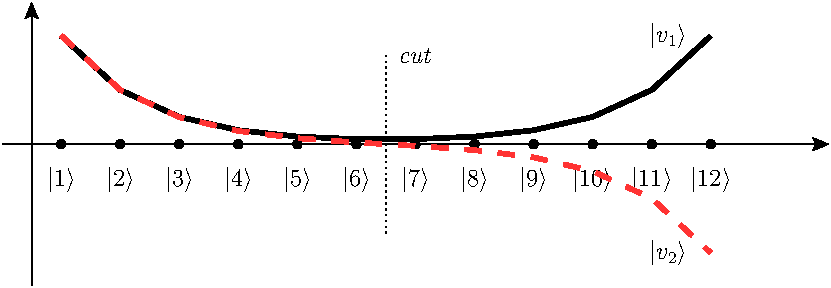
\includegraphics[]{pic-dwell.pdf}
\end{center}
The simplest way to show this model
is gapless is using a variational
argument.
Any another vector $\ket{u}$
that is orthogonal to the groundspace
vector will have $\bra{u}H\ket{u} \le \lambda_2.$
To construct a candidate for $\ket{u}$
partition the
basis vectors into two parts:
$$
    \Gamma = \Gamma_A \cup \Gamma_B
$$
and write $\ket{v_1} = 
\ket{v_A}\oplus\ket{v_B}$
and write the Hamiltonian with this
decomposition as
$$
H = 
\left(\begin{array}{ll}
H_{AA} & H_{AB} \\
H_{BA} & H_{BB}
\end{array}\right).
$$
Now let
$$
    \ket{u} = \ket{v_A} \oplus -\ket{v_B}
$$
%$$
%\braket{i}{u} =
%    \left\{ \begin{array}{ll}
%     +\braket{i}{v_1} &\mbox{if}\ \ket{i}\in\Gamma_A \\
%     -\braket{i}{v_1} &\mbox{if}\ \ket{i}\in\Gamma_B\end{array}\right..
%$$
And then
\begin{align*}
    \lambda_2 \ge \bra{u}H\ket{u} &= 
\bra{v_A}H_{AA}\ket{v_A} +
\bra{v_B}H_{BB}\ket{v_B} -
\bra{v_B}H_{BA}\ket{v_A} -
\bra{v_A}H_{AB}\ket{v_B} \\
    &= \lambda_1 - 4 \bra{v_B}H_{BA}\ket{v_A}.
\end{align*}
So if we can show that 
$ \bra{v_B}H_{BA}\ket{v_A}$
tends to zero we are done.
This term involves the 
dynamical coupling between the
groundstate wavefunction along
the ``cut'' between $A$ and $B$.
To succeed we must find such a cut where
the wavefunction is small. In general
this appears to be quite difficult,
even though in the models we are considering
numerics show that not only is the
wavefunction small away from potential wells
but it is exponentially small.

In summary, we note the important
features of this model.
The groundstate wavefunction has all
positive components, which implies
that the size of the gap is controlled
by the ``weight'' of a cut.
Also, we are hinting at the role
of symmetry as these cuts will
turn out to be reflection lines
under certain symmetries of the models
we consider.

\subsection{Perron-Frobenius structure theory}

%We restrict our attention to Hamiltonians whose off-diagonal entries
%are non-negative (in some basis).
%These are also known as \emph{stoquastic} Hamiltonians \cite{Bravyi2006}.
%This can be achieved by considering Hamiltonians where each term
%involves either $X$-type operators or $Z$-type operators but not both.
%That is, $G_0$ consists only of $X$-type operators and $Z$-type operators.
%We will call this a \emph{CSS gauge code Hamiltonian} after the stabilizer codes
%of the same name.
%We also shift the Hamiltonian by a constant energy, so that
%the diagonal entries are non-negative:
%$$
%%\Ham := \sum_{g\in G_0} \rho_{\mathrm{pauli}}(g).
%\Ham := \sum_{g\in G_0} \rho_{\mathrm{pauli}}(g) + kI.
%$$
%This does not change the spectral gap or eigenvectors.

%This is another kind of representation theory of $\Pauli_n.$
%We are representing either $G_X$ or $G_Z$ as a permutation representation (?)
%It has the ability to extract irreps of $G$ corresponding to
%the $X$ type operators as affine subspaces $\{vR_X+t\}$ of $\Fn.$
%For the $Z$ representations we will still need the complex
%representation theory to build states on $\Complex[\{vR_X+t\}]$
%that look like ``waves''.
%These (stationary) waves do indeed have a geometric interpretation,
%with the wavefront nodes being identified with so-called Cheeger cuts.
%To switch back and forth between the $X$ and $Z$ type
%representations 

%See \cite{Baez2012}
We return to the investigation of Hamiltonians
formed from CSS gauge codes.
We can think of such Hamiltonians as the adjacency matrix of a graph.
The diagonal terms (working in the computational basis)
come from the $Z$ operators and the off-diagonal terms
come from $X$ type operators.
Loosely speaking we can view the off-diagonal terms as 
raising and lowering operators, and the diagonal
terms measure the energy of each level.

The off-diagonal entries are all positive, and
if we use a spectral shift operator ($+cI$) we
find that $H+cI$ is a non-negative matrix and
now we can use the Peron-Frobenius theorem.

An irreducible matrix is ... 
% https://en.wikipedia.org/wiki/Perron%E2%80%93Frobenius_theorem#Non-negative_matrices

\begin{framed}
In the computational basis, any CSS gauge code
Hamiltonian $H$ is the direct sum of $2^{m_Z}$
irreducible matrices $\Gamma_{t_X}$
indexed by $t_X\in\Span{T_X}$
with multiplicity $2^k$:
$$
    H = \bigoplus_{
    \substack{t_X\in\Span{T_X}\\l_X\in\Span{L_X}}}
        \Gamma_{t_X}.
$$
\end{framed}

Each of these blocks $\Gamma_{t_X}$ is also Perron-Frobenius
and this means the following:
\begin{framed}
For each $t_X\in\Span{T_X}$
the largest eigenvalue 
of $\Gamma_{t_X},$
$$\lambda_1(\Gamma_{t_X})
$$
is non-degenerate,
and is associated with an eigenvector 
$$v_1(\Gamma_{t_X})
$$
with positive components.
\end{framed}

Now we make the restriction that $H$
comes from a weakly self-dual gauge code.
Our goal will be to show that the
groundspace of $H$ is spanned
by vectors which are stabilized.
This will imply that $\lambda_1(H)=\lambda_1(H_{0,0}).$
To begin, let $v_1$ be the top
eigenvector of $\Gamma_{t_X}$ with $t_X\in\Span{T_X}.$
Because $v_1$ has all positive components
it will be fixed by  any operator
$s\in\Span{S_Z}$.
To show that the $X$ type stabilizers
also fix $v_1$ 
we use weak self-duality
and see that by change of basis
we can swap the roles of the $X$ and $Z$ type operators.
\begin{framed}
\noindent{\bf Fact 1:}

For any weakly self-dual gauge code Hamiltonian $\Ham$
every groundstate is stabilized 
and so $$\lambda_1(\Ham) = \lambda_1(\Ham_{0,0})$$
and for $t_X\in\Span{T_X}, t_Z\in\Span{T_Z}$
with $t_X\ne 0$ or $t_Z\ne 0$
$$
\lambda_1(\Ham) > \lambda_1(H_{t_X,t_Z}).
$$
\end{framed}
Notice that 
$H_{0,0}$ is also Perron-Frobenius (in the computational basis)
and so has non-degenerate
groundspace, but it appears with multiplicity $2^k$ within
the Hamiltonian $H$ and this accounts for the degeneracy of the
groundspace of $H$.

%Taken together, these eigenvectors form a basis for the
%groundspace of the system.
%Stabilizers act as $+1$ or $-1$ on eigenvectors
%of the Hamiltonian.
%A stabilizer $s\in\Pauli^X$ just permutes the
%coordinates of the groundstate and so must fix any
%groundstate. 
%A stabilizer $s\in\Pauli^Z$ acts trivially
%on $\ket{0...0}$ and therefore must also fix any groundstate.
%We have demonstrated the following

%A simple variational argument % ???
%shows that the top eigenvector (the groundstate)
%can be chosen to have all positive entries
%(this is the Perron-Frobenius theorem)
%and therefore is stabilized:

The next goal is to search for
the second eigenvalue of $H$,
$\lambda_2(H).$

Using a basis change and the
above equation (???) for $H_{t_X,0}$
we have
\begin{framed}
\noindent{\bf Fact 2:}

Given a weakly self-dual
gauge code Hamiltonian $\Ham$ and
$t_X\in \Span{T_X},\  t_X\in \Span{T_Z}$
the blocks $\Ham_{t_X,0}$ and 
$\Ham_{0,t_Z}$ are Perron-Frobenius.
\end{framed}

We extend the above argument:
\begin{framed}
For a weakly self-dual gauge code
Hamiltonian,
and $t_X\ne 0$, $t_Z\ne 0$
\begin{align*}
\lambda_1(\Ham_{t_X,0}) &< 
    \lambda_1(\Ham_{t_X,t_Z}) \ \mbox{and}\\
\lambda_1(\Ham_{0,t_Z}) &< 
    \lambda_1(\Ham_{t_X,t_Z}).
\end{align*}
\end{framed}

The following fact would appear to
be true under certain conditions,
but is not at all true
for example when $T$ is trivial.
\begin{framed}
\noindent{\bf Proto-fact:}

For a sufficiently ``well-behaved''
weakly self-dual
gauge code Hamiltonian $H$
\begin{align*}
\lambda_2(\Ham) 
    &= \min_{t_X\ne 0} \lambda_1(\Ham_{t_X,0})\\
    &= \min_{t_Z\ne 0} \lambda_1(\Ham_{0,t_Z}).
\end{align*}
%for some
%$(t_X,t_Z) \ne (0, 0).$
\end{framed}

\subsection{Cheeger inequalities}

In \cite{Friedland2002}, they derive the following Cheeger inequality
by considering bi-partitions of the graph. We will do the
same, but using matrix block notation.

Let $v_2$ be a second eigenvector, $ \Ham v_2 = \lambda_2 v_2 $ 
and $||v_2||=1$.
We bi-partition the space 
so that $v_2$ has (vector) blocks:
$$
v_2 = \left( \begin{array}{l}
x\\
y\end{array} \right)\quad
$$
with $x\ge 0$ and $y\le 0,$ component-wise.
Let the blocks of $\Ham$ under the same partition be:
$$
\Ham = \left( \begin{array}{ll}
A&C\\
C^\top&B\end{array} \right).\quad
$$
If we denote $\lambda_1(A)$ as the top eigenvalue of $A$ and
$\lambda_1(B)$ as the top eigenvalue of $B$,
then
\begin{align*}
\lambda_2 = v_2^\top \Ham v_2 &= x^\top A x + 2 x^\top C y + y^\top B y \\
        &\le x^\top A x + y^\top B y\ \le\ ||x||^2 \lambda_1(A) + ||y||^2 \lambda_1(B) \\
        &\le \mbox{min}(\lambda_1(A), \lambda_1(B))\ \le\ \lambda_1.
\end{align*}

Defining the following constant as a maximisation over
all bi-partitions of $\Ham:$
$$
    \nu(\Ham) := \max_{A, B}\ \mbox{min}(\lambda_1(A), \lambda_1(B))
$$
the above calculation shows that
$$
    \lambda_2 \le \nu(\Ham) \le \lambda_1.
$$

To bound $\lambda_2$ from below, we use a variational argument.
For any unit vector $v$ orthogonal to the top eigenspace of $\Ham$ we
have $v^\top \Ham v \le \lambda_2.$


%%%%%%%%%%%%%%%%%%%%%%%%%%%%%%%%%%%%%%%%%%%%%%%%%%%%%%%%%%%%%%%%%%%%%%%%%%%%%%%
%

\subsection{The compass model is gapless}

Although there is strong evidence that the gap dissapears as the lattice size
$l$ grows, it is still worthwhile considering the exact reasons for this.

We use a variational argument to show that $\lambda_1(H_{t_X,0})$
is close to $\lambda_1(H_{0,0}).$
Given the similarity of the form of these two blocks, we
take the ground eigenvector $v_1$ of $H_{0,0}$ and apply it
to $H_{t_X,0}$. % where $t_X$ has low weight.
Recall that we identified the bases of these two Hamiltonian blocks.
\begin{align*}
    \lambda_1 - \lambda_2 &\le \bra{v_1}H_{0,0}\ket{v_1} - \bra{v_1}H_{t_X,0}\ket{v_1}  \\
            &= \bra{v_1}(H_{0,0} - H_{t_X,0})\ket{v_1}  \\
    &= \sum_{v\in\Fr} 2\bigl(w(G_Z R_X^\top v^\top + G_Z t_X^\top) -w(G_Z R_X^\top v^\top)\bigr) 
    |\braket{v}{v_1}|^2.
\end{align*}

FAIL

%%%%%%%%%%%%%%%%%%%%%%%%%%%%%%%%%%%%%%%%%%%%%%%%%%%%%%%%%%%%%%%%%%%%%%%%%%%%%%%
%

\subsection{Perturbation of the Perron vector}

Lemma:
Let $A$ be non-negative irreducible $n\times n$ matrix.
Let $v\ne 0$ be a non-negative $n$ vector, and $B = A + \ket{e_i}\bra{v}.$
Then 
$$
\frac{y_i}{x_i} > \frac{y_j}{x_j} \ \ \mbox{for}\ \ j \ne i,
$$
where $x, y$ are the Perron eigenvectors of $A, B$ respectively
\cite{Elsner1982}.

Let $H(t)$ be non-negative irreducible matrix, continuously
differentiable wrt $t.$
Let $v(t)$ and $\lambda(t)$ be the Perron eigenvector and value of $H(t)$
with $\braket{v}{v}=1.$
Then
$$
    \lambda' = \bra{v}H'\ket{v}
$$
and
$$
    \ket{v'} = -(H-\lambda)^{-1}(H' - \lambda')\ket{v}.
$$
where $(H-\lambda)^{-1}$ is the Moore-Penrose inverse of $H-\lambda.$ See \cite{Meyer1988}.



%%%%%%%%%%%%%%%%%%%%%%%%%%%%%%%%%%%%%%%%%%%%%%%%%%%%%%%%%%%%%%%%%%%%%%%%%%%%%%%
%

\subsection{Numerics}

% !!!                                              !!!
% !!!                                              !!!
% !!! note we use 1-based row indices for T_X here !!!
% !!!                                              !!!
% !!!                                              !!!
\begin{center}
\begin{tabular}{ c|c|c|c|c|cc|c } 
model       & $n$ &  $t_X$    & $w(s_X)$ & $\lambda_1$ & $\lambda_2$ ?&  & gap \\
\hline
\hline
gauge color & 15  & 0         & &  25.455844  & 16.970563   & &  \\
            &     & $T_X(1)$  & 8 &              & 22.214755 &\checkmark & 3.241089           \\
%           &     &           & &              &              &            \\
\hline
gauge color & 39  & 0         & &  64.476081   & 58.137233   & &  \\
            &     & $T_X(1)$  & 8 &              & 60.706477   & &   \\
            &     & $T_X(2)$  & 12 &              & 61.366348  & &  \\
            &     & $T_X(3)$  & 8 &              & 60.357053 & &    \\
            &     & $T_X(10)$  & 20 &              & 63.495916 & \checkmark  & 0.980165 \\
\hline
gauge color & 65  & 0         & &  104.076     & 98.8 $\pm$1 &  &    \\
            &     &  $T_X(1)$ & 18 &              &  102.382   & \checkmark  &  1.694 \\
            &     &  $T_X(3)$ & 12 &              &  100.585   &  &            \\
            &     &  $T_X(4)$ & 8  &              &  100.4  &  &            \\
            &     &  $T_X(8)$ & 12 &              &  101.6 &  &            \\
\end{tabular}
\end{center}

\begin{center}
\begin{tabular}{ c|c|c|c|c|cc|c } 
model       & $n$ &  $t_X$    & $w(s_X)$ & $\lambda_1$ & $\lambda_2$ ?&  & gap \\
\hline
\hline
compass $l=4$ & 16  &   0        &   &  19.012903&    16.335705     &     &            \\
              &     &   $T_X(1)$ & 8 &              &  18.369300    &\checkmark & 0.643603 \\
\hline
compass $l=5$ & 25  &   0        &   & 29.076200 & 27.597280   &     &            \\
              &     &   $T_X(1)$ & 10 &              & 28.624004 &\checkmark &  0.452196 \\
\hline
compass $l=6$ & 36  &   0        &   & 41.410454 & 40.585673   &     &            \\
              &     &   $T_X(1)$ & 12 &              & 41.094532 &\checkmark &  0.315922 \\
%             &     &           &   &              &          &    &            \\
\end{tabular}
\end{center}

We use the iterative solvers in software library {\tt SLEPc} \cite{Hernandez2005} to find these
eigenvalues.

%%%%%%%%%%%%%%%%%%%%%%%%%%%%%%%%%%%%%%%%%%%%%%%%%%%%%%%%%%%%%%%%%%%%%%%%%%%%%%%
%

\subsection{The orbigraph}

A graph automorphism is a permutation matrix $P$
such that $P^T \Ham P = \Ham$.
Equivalently, $P$ commutes with $\Ham$ and this means it preserves
the eigenspaces of $\Ham$.
%To show $P$ acts trivially on the groundstate we
%need to check that it commutes with the logical
%operators.

\def\auto{A}
\def\smbox#1{\ \ \mbox{#1}\ \ }
The set of all such graph automorphisms 
form a group $\auto$.
We now define a new matrix $\Ham//\auto$
that acts on the vector space with basis consisting
of the orbits of $\auto.$
%The groundspace wavefunction is constant
%on each $\auto-$orbit.
%The top eigenvalue of $\Ham//\auto$ will be the
%same as the top eigenvalue of $\Ham.$

The matrix components of $\Ham//\auto$ will be
$$
    (\Ham//\auto)_{ij} = |\{ g\in G \smbox{s.t.} gv \in j \}| \smbox{for some}v\in i
$$
for each pair of $\auto-$orbits $i$ and $j$.
In other words, 
$(\Ham//\auto)_{ij} $ counts the number of gauge group
elements that sends any particular element $v$ of the 
$\auto-$orbit $i$ to the $\auto-$orbit $j.$

Here is a simple example. % potential only depends on hamming weight: Jarret
We take as gauge group 
$$G = \{XII, IXI, IIX, ZII, IZI, IIZ\}.$$
The Hamiltonian $H = \sum_{g\in G} g$ has matrix:
$$
H = \left(\begin{array}{rrrrrrrr}
 3 &  1 &  1 &  1 &  0 &  0 &  0 &  0 \cr
  1 &  1 &  0 &  0 &  1 &  1 &  0 &  0 \cr
  1 &  0 &  1 &  0 &  1 &  0 &  1 &  0 \cr
  1 &  0 &  0 &  1 &  0 &  1 &  1 &  0 \cr
  0 &  1 &  1 &  0 & -1 &  0 &  0 &  1 \cr
  0 &  1 &  0 &  1 &  0 & -1 &  0 &  1 \cr
  0 &  0 &  1 &  1 &  0 &  0 & -1 &  1 \cr
  0 &  0 &  0 &  0 &  1 &  1 &  1 & -3
\end{array}\right)
$$
In this case, the automorphism group is $\auto=S_3,$
there are four $\auto-$orbits, and
$$
H//\auto = \left(\begin{array}{rrrr}
 3 &  3 &  0 &  0 \cr
  1 &  1 &  2 &  0 \cr
  0 &  2 & -1 &  1 \cr
  0 &  0 &  3 & -3
\end{array}\right).
$$
In this case the automorphism group $\auto$ of the graph
is the same as the automorphism group $Aut(G)$ of the gauge group,
but in general it is possible that $Aut(G) < \auto.$

Note that the orbigraph is no longer Hermitian,
and in general will not even be normal.

We can also write $H//A = QHP$ using the following two matrices for $P$ and $Q:$
$$
Q = 
\left(\begin{array}{rrrrrrrr}
 1 &  0 &  0 &  0 &  0 &  0 &  0 &  0 \cr
  0 &  1 &  0 &  0 &  0 &  0 &  0 &  0 \cr
  0 &  0 &  0 &  0 &  1 &  0 &  0 &  0 \cr
  0 &  0 &  0 &  0 &  0 &  0 &  0 &  1
\end{array}\right),\ \ \ 
P = 
\left(\begin{array}{rrrr}
 1 &  0 &  0 &  0 \cr
  0 &  1 &  0 &  0 \cr
  0 &  1 &  0 &  0 \cr
  0 &  1 &  0 &  0 \cr
  0 &  0 &  1 &  0 \cr
  0 &  0 &  1 &  0 \cr
  0 &  0 &  1 &  0 \cr
  0 &  0 &  0 &  1
\end{array}\right).
$$
The idea is that each column of $P$ sums over an orbit,
and each row of $Q$ chooses one member of each orbit.

The automorphisms of the gauge group, $Aut(G)$ will induce an
automorphism of the graph by ...
In particular, elements of the stabilizer group $\Stab$ induce graph 
automorphisms by ...
In general there may be more symmetry in the graph that
we cannot access via a group automorphism.

See also \cite{Cvetkovic1980} chapter 5.

In general, we will apply this idea to each of the blocks $H_t$.
From {\bf Fact 2} above, and using the fact that we are
summing over a trivial representation of $Aut(G)$ we have the following:
\begin{framed}
\noindent{\bf Fact 3:}

The orbigraph of $\Ham_{0,0}$ contains the ground eigenvalue of $\Ham_{0,0}.$
\end{framed}

%%%%%%%%%%%%%%%%%%%%%%%%%%%%%%%%%%%%%%%%%%%%%%%%%%%%%%%%%%%%%%%%%%%%%%%%%%%%%%%
%
\subsubsection{Compass model}
For the next example we take the $l=3$ compass model.
$\Ham_{0,0}$ acts on a 16 dimensional space.
The order of $A$ is $72$, and we find three $A-$orbits.
% This time $Aut(G) = A$ ???
The orbigraph method can be applied in the case
where the Hamiltonian weights for $X$ and $Z$ are uniform as $w_X$ and $w_Z.$
We separate the $X$ and $Z$ terms of the orbigraph to show
how this works:
$$
\Ham_{0,0}//\auto = 
\left(\begin{array}{rrr}
 0 &  9 &  0 \cr
  1 &  4 &  4 \cr
  0 &  6 &  3
\end{array}\right) + 
\left(\begin{array}{rrr}
 9 &  0 &  0 \cr
  0 &  1 &  0 \cr
  0 &  0 &  -3
\end{array}\right)
=
\left(\begin{array}{rrr}
 9 &  9 &  0 \cr
  1 &  5 &  4 \cr
  0 &  6 &  0
\end{array}\right)
$$
This can be solved analytically and we find $\lambda_1 = 4+2\sqrt{13} \cong 11.21110255.$
Keep in mind that the original state space has dimension $2^9=512$ so we
have come a long way down to 3.

By exact\footnote{Exact in this context means that we do not do any
perturbative approxiamations to the operator in question.}
numerical diagonalization
we get the spectrum of $\Ham_{0,0}$ and note that the orbigraph lifts
all degeneracy as well as missing some excited eigenspaces:
\begin{center}
\begin{tabular}{ c|c|c } 
$\lambda$ & $\Ham_{0,0}$ degeneracy & $\Ham_{0,0}//A$ degeneracy \\
\hline
    11.2111025509 & 1 & 1 \\
    6.0 & 1 & 1 \\
    2.0 & 4 &   \\
    0.0 & 4 &   \\
    -3.21110255093 & 1 & 1 \\
    -4.0 & 4 &   \\
    -6.0 & 1 &   
\end{tabular}
\end{center}
The reason we miss some excited spaces is that they do not contain
any trivial irrep of $A.$
Note that we miss the eigenspace with $\lambda = -6$
even though this is one dimensional. It must contain some other non-trivial
one dimensional irrep. This cannot happen with the groundspace because
those eigenvectors are all positive.

If we want to make an orbigraph for these other spaces we would construct
the orbigraph by
summing over orbits using different characters of $A$
(these are \emph{momenta} in the abelian terminology).
See \cite{Cvetkovic1980} chapter 5 for more details.

%%%%%%%%%%%%%%%%%%%%%%%%%%%%%%%%%%%%%%%%%%%%%%%%%%%%%%%%%%%%%%%%%%%%%%%%%%%%%%%
%
\subsubsection{Gauge color code model}
The Gauge color code \cite{Bombin2015,Bombin2015single}...
This is a self-dual code...
The smallest in the ensemble has $n=15$ qubits,
$G_0$ has $18$ each of X/Z-type gauge operators,
and $4$ each of X/Z-type stabilizer generators.
$\Ham_{0,0}$ acts on a 64 dimensional space, and $A$ has
order 720, and we find 7 orbits:
$$
\Ham_{0,0}//\auto = 
\left(\begin{array}{rrrrrrr}
18 & 18 &  0 &  0 &  0 &  0 &  0 \cr
  3 & 12 & 15 &  0 &  0 &  0 &  0 \cr
  0 &  6 &  6 & 12 &  0 &  0 &  0 \cr
  0 &  0 &  9 &  0 &  9 &  0 &  0 \cr
  0 &  0 &  0 & 12 & -6 &  6 &  0 \cr
  0 &  0 &  0 &  0 & 15 & -12 &  3 \cr
  0 &  0 &  0 &  0 &  0 & 18 & -18
\end{array}\right)
$$
The eigenvalue equation results in
the recurrence relation:
$$
    \lambda a_k = 3ka_{k-1} + (18-6k)a_k + (18-3k)a_{k+1},
$$
which has largest solution 
$\lambda_1 = 18\sqrt{2} \cong 25.4558441.$

% RP^3 is homeomorphic to the solid ball with antipodal points identified
% http://math.stackexchange.com/questions/507783/mathbbrp3-is-homeomorphic-to-the-solid-ball-with-antipodal-points-identifi
% http://topospaces.subwiki.org/wiki/Homology_of_real_projective_space

Numerics give the full spectrum of $\Ham_{0,0}$ and we note that the orbigraph lifts
all degeneracy as well as preserving every eigenvalue:
\begin{center}
\begin{tabular}{ c|c|c } 
$\lambda$ & $\Ham_{0,0}$ degeneracy & $\Ham_{0,0}//A$ degeneracy \\
\hline
    25.4558441227 & 1 & 1 \\
    16.9705627485 & 6 & 1 \\
    8.48528137424 & 15 & 1 \\
    0.0 & 20 & 1 \\
    -8.48528137424 & 15 & 1 \\
    -16.9705627485 & 6 & 1 \\
    -25.4558441227 & 1 & 1 \\
\end{tabular}
\end{center}

The second eigenvalue of $H$ comes from a recurrence
relation in two variables which has solution
$\lambda_2 = 9\sqrt{2} + 3\sqrt{10} \cong 22.21475504.$
So the gap for this Hamiltonian  is 
$$\lambda_1 - \lambda_2 = 9\sqrt{2} - 3\sqrt{10} \cong 3.24108908.$$


%%%%%%%%%%%%%%%%%%%%%%%%%%%%%%%%%%%%%%%%%%%%%%%%%%%%%%%%%%%%%%%%%%%%%%%%%%%%%%%
%
\subsubsection{A table of orbigraphs}

Here we tabulate some automorphisms of $H_t$
and resulting orbigraph sizes.

We define a group of symmetries of the code as...

\begin{center}
\begin{tabular}{ c|c|c|c|c|c|c } 
model &\ $n$\ &\ $r$\ &\ $t_X$\ & $|A|$ & orbits & Aut(code) \\
\hline
    xy & 4 &  2& 0 & 2 & 3 & 8 \\
       & 5 &  4& 0 & 10 & 4 & 10 \\
       & 6 &  4& 0 & 72 & 3 & 12 \\
       & 7 &  6& 0 & 14 & 9 & 14 \\
       & 8 &  6& 0 & 4608 & 10 & 16 \\
       & 9 &  8& 0 & 18 & 23 & 18  \\
       & 10 & 8& 0 & 200 & 10 & 20  \\
    %   & 11 & & 0 & 22 & 63 & 22  \\
    %   & 12 & & 0 & 288 & 36 & 24  \\
\hline
    compass $l=3$ & 9 & 4 & 0 & 72 & 3 & 36 \\
                  & 9 & 4 & $t_X$ & 12 & 4 &  \\
            $l=4$  & 16 & 9  & 0 & 128 & 24 & 64 \\
                   & 16 & 9  & $t_X$ & 16 & 48 &  \\
            $l=5$  & 25 & 16 & 0 & 200 & 430 & 100 \\
                   & 25 & 16 & $t_X$ & 20  & 3418 &  \\
\hline
    gauge color & 15 & 6  & 0 & 720 & 7 & 24  \\
                & 15 & 6  & $t_X$ & 36 & 16 &  \\
                & 39 & 18 & 0 & 36 & 14400 & 3  \\
                & 65 & 32 & 0 & ?? & ?? & 4 \\
\end{tabular}
\end{center}

From this table it looks like $H_{0,0}$ for the compass model $|A| = 8l^2.$

Note that for large graphs, numerically finding the orbigraph has comparable
difficulty to just (numerically) solving the original eigenvalue problem.

We use the software library {\tt nauty}\cite{McKay2014} for computing graph automorphisms.


%%%%%%%%%%%%%%%%%%%%%%%%%%%%%%%%%%%%%%%%%%%%%%%%%%%%%%%%%%%%%%%%%%%%%%%%%%%%%%%
%
%%%%%%%%%%%%%%%%%%%%%%%%%%%%%%%%%%%%%%%%%%%%%%%%%%%%%%%%%%%%%%%%%%%%%%%%%%%%%%%
%


\subsection{Discussion}

In \cite{AlShimary2010}, they 
build a kind of graph laplacian from a known ground state:
``This is not a major drawback as there
are large families of physically relevant states, e.g. the
Matrix Product States, that are ground states of Hamil-
tonians which are not known to be gapped or not in two
or higher dimensions. Such an important example is
the two-dimensional AKLT model that can support uni-
versal quantum computation by measurements only, but
it is not proven yet if it is gapped which would establish
its fault-tolerance.''
This Laplacian has the same gap as the Hamiltonian.

It would be nice to connect geometric properties of the
graph to spectral gap properties. For example, the spectral gap of
the normalized graph laplacian can be bounded from below
by the Coarse Ricci curvature \cite{Lin2011}. 
Unfortunately, it appears
that there are no good connections between the spectrum
of the normalized graph laplacian and the spectrum of the adjacency matrix.
% http://mathoverflow.net/questions/118870/connection-between-eigenvalues-of-matrix-and-its-laplacian

See also \cite{Jarret2014,Jarret2015}. 
In \cite{Jarret2015modulus} they
write the Hamiltonian as a sum of the
the combinatorial graph Laplacian and a (diagonal) potential, 
and then employ methods from PDE theory \cite{Andrews2011}.
Also: \cite{Baume2016}. % Michaels' Phd thesis

We expect generic local hamiltonians to be gapless \cite{Movassagh2016}.

%%%%%%%%%%%%%%%%%%%%%%%%%%%%%%%%%%%%%%%%%%%%%%%%%%%%%%%%%%%%%%%%%%%%%%%%%%%%%%%
%
%%%%%%%%%%%%%%%%%%%%%%%%%%%%%%%%%%%%%%%%%%%%%%%%%%%%%%%%%%%%%%%%%%%%%%%%%%%%%%%
%

\section{Outlook}

There's a growing zoo of these systems and little is known
about their energetics, in particular if they are gapped or
not as the size increases.

A family of topological subsystem codes,
from the code perspective  \cite{Bombin2010,Bombin2014,Suchara2011},
from the cond-mat (integrals of motion!) perspective:
\cite{Kargarian2010,Bombin2009}
Topological subsystem Codes: \cite{Suchara2011}
Structure of 2D Topological Stabilizer Codes: \cite{Bombin2014}
Gauge color codes, gauge fixing: \cite{Bombin2015}
Gauge color codes, single shot: \cite{Bombin2015single}

A generalization of this is the 
monomial formalism \cite{Van2011}. 
These operators also form a group and would
have a corresponding representation theory.


%% CUT HERE
%\appendix
%% CUT HERE

%\label{appendix}

% CUT HERE

\bibliography{refs}{}
\bibliographystyle{abbrv}


\end{document}


